% Michal Kovac's master thesis
%
\documentclass[a4paper,12pt]{book}
\usepackage{pgf}
\usepackage[utf8]{inputenc}
%\usepackage{a4wide}
%% Now, switch on what is appropriate for czech:

% czech quotation marks
% \bq - begin quotation, \eq - end quotation
\def\bq{\mbox{\kern.1ex\protect\raisebox{-1.3ex}[0pt][0pt]{''}\kern-.1ex}}
\def\eq{\mbox{\kern-.1ex``\kern.1ex}}
%\setlanguage{\czech}

{%                                      % Begin a group for which " is active
\catcode`\"=\active                     % Make " an active character
\catcode`\@=11                          % Make @ an active character
%
%  \csdoublequoteson
%
%       This macro makes " an active character, resets the control sequence
%       \dblqu@te to L (left), and defines \dq as a replacement for ".
%
\gdef\csdoublequoteson{%                % \csdoublequoteson enables "
    \gdef"{\czechquotes}%               % Define " as \czechquotes
    \global\catcode`\"=\active%         % Make " an active character
    \global\chardef\dq=`\"%             % Double-quote char. via \dq
    \global\let\dblqu@te=L%             % Always start with a left double-quote
    }                                   % End of macro
%
%  \bq, \eq
%
%      These macros define default characters for czech left and right
%      double quotes. Czech opening quote is created from two commas with
%      kerning depending on fontdimen four parameter of current font.
%      Better solution should be specially designed character with
%      proper kernings; if you have such characters in fonts
%      (e.g. in DC-fonts), use it instead. (e.g. define
%      macros \bq and \eq e.g. \def\bq{\char"130 }
%      in your document/style file-- not in csquote.sty!)
%      Similar solution is used for czech right quote.
%
%      \cs existence test, stolen from TeXbook exercise 7.7
\def\ifundefined#1{\expandafter\ifx\csname#1\endcsname\relax }%
%
%      another macro to be more efficient in time and space
\global\chardef\f@@r=4
%
\ifundefined{bq}%
\gdef\bq{\kern-.25\fontdimen\f@@r\font,\kern-.8\fontdimen\f@@r\font,%
                \kern-.35\fontdimen\f@@r\font}%
\fi
\ifundefined{eq}%
\gdef\eq{\kern-.35\fontdimen\f@@r\font`\kern-.8\fontdimen\f@@r\font`%
                \kern-.25\fontdimen\f@@r\font}
\fi
%
% Macro \uv for other usage of \bq and \eq.
%
\ifundefined{uv}%
        \gdef\uv#1{\bq #1\eq}
\fi
%
% \testquotes macro gives warning if citation span this place
%
\gdef\testquotes{\if R\dblqu@te
        \message{Warning: You forgot right double quote!}%
        \let\dblqu@te=L\fi}
%
%  Define the macro that will be executed whenever " is encountered.
%
\gdef\czechquotes{\protect\czechqu@tes}
\gdef\czechqu@tes{%
        %  If the double-quote is the first character in a new paragraph,
        %  make sure it becomes a left double-quote.  This case can be
        %  detected by checking to see if TeX is currently in vertical mode.
        %  If so, the double-quote is at the beginning of the paragraph
        %  (since " hasn't actually generated any horizontal mode tokens
        %  yet, TeX is still in vertical mode).  If the mode is vertical,
        %  set \dblqu@te equal to L.
        %
        \ifinner\else\ifvmode\testquotes\fi\fi%
        %
        %  Now insert the appropriate left or right double-quote.
        %
        %  If \dblqu@te is L, insert an opening quote and set \dblqu@te to R.
        %
        \if L\dblqu@te\bq\global\let\dblqu@te=R%
        %
        %  Otherwise, save the current \spacefactor, insert '', set \dblqu@te
        %  to L, and reset the original \spacefactor.
        %
        \else%
           \let\xxx=\spacefactor%               % Save the \spacefactor
           \eq%                                 % Insert ending quote
           \global\let\dblqu@te=L%              % and reset \dblqu@te
           \spacefactor\xxx%                    % Reset the \spacefactor
        \fi%                                    % End of \if L\dblqu@te...
        }                                       % End of " macro
}                                               % End of group

\gdef\csdoublequotesoff{%
        \catcode`\"=12%                         % Set " back to other
        }
%
% Czech quotes are default
%
\csdoublequoteson



\usepackage{hyperref}
\usepackage[czech,english]{babel}

%\pgfdeclareimage[interpolate=true,height=7cm]{faktorial}{faktorial}
%\pgfdeclareimage[interpolate=true,height=7cm]{designimage}{designB}
%\pgfdeclareimage[interpolate=true,height=3cm]{designimageSmall}{designB}
%\pgfdeclareimage[interpolate=true,height=3.5cm]{creatorFactoryimage}{creatorFactory}

\author{Michal Kováč}
\title{User-oriented language for solving KDD tasks}
%\date{\today}

\begin{document}
\selectlanguage{czech}
\begin{titlepage}
\begin{center}
\ \\

\vspace{15mm}

\large
Univerzita Karlova v Praze\\
Matematicko-fyzikální fakulta\\

\vspace{5mm}

{\Large\bf DIPLOMOVÁ PRÁCE}

\vspace{10mm}

%%% Aby vložní loga vše správně fungovalo, je třeba mít soubor logo.eps nahraný v pracovním adresáři,
%%% tj. v adresáři, kde se nachází překládaný zdrojový soubor. Soubor logo.eps je možné získat např.
%%% na adrese: http://www.mff.cuni.cz/fakulta/symboly/logo.eps

\includegraphics[scale=0.3]{logo}

\vspace{15mm}

%\normalsize
{\Large Michal Kováč}\\
\vspace{5mm}
{\Large\bf User-oriented language for solving KDD tasks}\\
\vspace{5mm}
Katedra softwarového inženýrství
\end{center}
\vspace{15mm}

\large
\noindent Vedoucí diplomové práce: doc. RNDr. Jan Rauch, CSc.
\vspace{1mm}

\noindent Studijní program: Informatika

\vspace{20mm}

\begin{center}
2008
\end{center}

\end{titlepage} % zde končí úvodní strana

\newpage

\normalsize % nastavení normální velikosti fontu
\setcounter{page}{2} % nastavení číslování stránek
\ \vspace{10mm}

\noindent !-- TODO poděkovat --!

\vspace{\fill}
Prohlašuji, že jsem svou diplomovou práci napsal samostatně a výhradně s použitím citovaných pramenů. Souhlasím se zapůjčováním práce.

\bigskip

\noindent V Praze dne \today \hspace{\fill}Michal Kováč\\

%%%   Výtisk pak na tomto míste nezapomeňte PODEPSAT!
%%%                                         *********
\selectlanguage{english}
\tableofcontents

\newpage
\selectlanguage{czech}
\begin{description}
 \item [Název práce:] Uživatelsky orientovaný jazyk pro řešení úloh DZD
 \item [Autor:] Michal Kováč
 \item [Katedra (ústav):] Katedra softwarového inženýrství
 \item [Vedoucí diplomové práce:] doc. RNDr. Jan Rauch, CSc.
 \item [E-mail vedoucího:] Rauch@vse.cz
 \item [Abstrakt:]
 \item [Klíčová slova:]
\end{description}
\selectlanguage{english}

\medskip

\begin{description}
 \item [Title:] User-oriented language for solving KDD tasks
 \item [Author:] Michal Kováč
 \item [Department:] Department of Software Engineering
 \item [Supervisor:] doc. RNDr. Jan Rauch, CSc.
 \item [Supervisor's e-mail address:] Rauch@vse.cz
 \item [Abstract:]
 \item [Keywords:]
\end{description}
%!--- MARTIN Nikde v obsahu jsem nenasel cast, ktera by srovnavala tvuj postup s jinymi moznymi postupy v DM ci jinde a srovnani v cem je to nase lepsi a horsi. Tohle tam hodne chybi ---
%!--- RE: problem je v tom, ze tu neni zadny alternativni postup, alespon me nic nenapada. Ja proste jen delam programivaci jazyk. Srovnani s jinymi jazyky se deje v ramci psani o tomtom jazyku pri jednotlivych featrach. Druhe misto, kde jsou alternativy jsou ty KDD priklady -- jejich reseni. Zase alternativy se diskutuji v ramci toho konkretniho prikladu. Ale samotne to, ze delam programovaci jazyk, nema alternativu -- co jineho by jsi chtel delat? ---!

\chapter{Introduction}
\section{Assignment}
\selectlanguage{czech}
Východiskem diplomové práce jsou zkušenosti s GUHA procedurami implementovanými v rámci systému LISp-Miner~\cite{GMGC}. Díky jak rozmanitosti vztahů které lze jejich pomocí hledat tak i vzhledem k rozsáhlým možnostem zadávání množiny potenciálně zajímavých vztahů lze pomocí těchto procedur hledat odpovědi na různé analytické otázky formulované způsobem blízkým přirozenému jazyku. Příkladem takové otázky je: „Za jakých okolností a pro které pacienty není pravda, že s rostoucí úrovní cholesterolu roste i úroveň trigliceridů?“ Na tuto otázku lze hledat odpovědi pomocí procedur 4ft-Miner, SD4ft-Miner, KL-Miner i SDKL-Miner. Použitá procedura i způsob nastavení jejích parametrů dává různé možnosti, co se týče podrobnosti odpovědi. Zevrubná odpověď na takovouto otázku vyžaduje několik vzájemně provázaných běhů několika procedur. Jednotlivé běhy procedur odpovídají dílčím otázkám indukovaným položenou otázkou.

Lze pokládat řadu podobných otázek které konstituují jistou typovou úlohu. Příkladem podobné otázky k otázce výše uvedené je otázka „Za jakých okolností a pro které pacienty není pravda, že s rostoucí úrovní vzdělání roste i spotřeba vína?“ Pro řešení jedné typové úlohy existuje systém vzájemně provázaných dílčích otázek a ty lze chápat jako příkazy vhodného jazyka, kterým uživatel řídí postup při řešení typové úlohy.

Jedná se o diplomovou práci kategorie „výzkumný problém“. Jejím cílem je stanovit několik typových úloh a pro ně definovat výše naznačený jazyk pro řešení. Jazyk bude založen na použití GUHA procedur implementovaných v rámci systému LISp-Miner, případně na nových vhodných analytických procedurách. Součástí diplomové práce bude i prototypová implementace příkazů tohoto jazyka v rámci systému FERDA~\cite{znalosti2006}.
\selectlanguage{english}

\section{Reaction to assignment}
%!--- MARTIN nove pojmy v teto i v dalsich sekcich by meli byt poprve kurzivou, potom uz normalne, at ctenar vi, ze je to neco noveho v textu a ne nejaky common knowledge ---
%Re: pracuji na tom

The main task of this thesis is to assess a set of several problems in KDD and to present a possible solution via a new user-oriented language for the Ferda system. The reach of the present thesis, however, surpasses the assignment in its implications. Instead of a new language specific only for some KDD problems, a new generic language with much wider extensibility and usability has been created as a part of this thesis. The reason for going beyond the task was the author's determination to present a more complex solution to the problem given. 

Instead of presenting first the KDD problems and later describing a new language specific for these problems a new generic language is introduced at the beginning. The language resulted indeed from some KDD problems but the language has been generalised for wider usage, which is why it is not needed to start with examples in this thesis.

The creation of a new more generic language independent of KDD was established as the first task, followed by demonstration of KDD problems and their solution using the generic language and special KDD functions in addition. The method used for creation of the new language relied on the principles of other functional languages, while maintaining the basic requirements of recursive enumerability and the widest possible application on the KDD problems.

%!--- MARTIN vysvetlit asi trosku lip, ctenar nemusi tusit co to je Ferda nebo LISp. Myslim ze Rauch k tomuto odstavci bude mit pripominky :) ---
%!--- RE: cilem tohoto odstavce neni aby ctenar chapal, co je LISp ci Ferda, jen aby pochopil, ze z nejakeho chytreho duvodu "neni splneno" zadani - vlastne je to jen oprava zadani - ve kterem taky neni vysvetleno, co to je LISp ci Ferda ---!

The new implementation of GUHA procedures that has been created as a part of \cite[diploma thesis of Tomáš Kuchař]{thesisKuchar} is used instead of LISp-Miner procedures which have been proposed. The new implementation of GUHA procedures is more generic and better integrated into the Ferda system. Use of the LISp-Miner procedures has been removed from the Ferda system.

\section{Structure}
The thesis is divided into five chapters. The first chapter discusses assignment of the thesis and guides to a solution of the assignment and the structure of the thesis.

The second chapter describes the Ferda system. Firstly, it discusses the history of Ferd and describes basics of the Ferda system including its functional view. Subsequently, it presents some details of its implementation. The chapter shows that Ferda was from beginning designed for user-oriented functional programming and describes what was missing in the Ferda system from the perspective of programming and extensibility before this thesis.

The third chapter goes into more detail and describes new features, functions and tools which make Ferda a strong user-oriented programing tool. Big amount of work is hidden in this chapter. To start with, it focuses on source files, the basic programming instrument, and how they are organized and how a code can be reused. Then several new basic functions are introduced with description of their pilot implementation. Modern programing methods are discussed in the last part of this chapter. Neither this chapter nor the first chapter are specifically oriented on knowledge discovery or data mining.

The fourth chapter realizes the main part of the assignment. It shows examples from KDD and presents how it can be solved in the Ferda system by functionalities introduced in the first two chapters. It also proposes new functionalities specific for KDD. The new features in the language are referenced from this chapter whenever they are used. Therefore it is possible to read this chapter before the previous, but it is not recommended for understanding the new language.

The last chapter summarizes previous chapters. It lists features which have been implemented as part of this thesis and features which have been only proposed.

\chapter{Basics of Ferda}
This chapter describes the Ferda system. First, it discusses the history of Ferda and basics of the Ferda system. Subsequently, it presents Ferda as a programming language. The latter part is important for understanding of the next chapter where Ferda is extended. The section shows that Ferda was designed from beginning for user-oriented functional programming and describes what was missing in the Ferda system from programming and extensibility before this thesis. It presents also formalization of the language, which can help with understanding the system and it describes how to transform a code in the language (which is graphical configuration of elements) to a text, which will be called ``textual representation''. The textual representation is used in the next chapters. Lastly, the chapter presents some details of implementation of the Ferda system. It can help programmers of extensions to the system, but it is not necessary for understanding of the thesis. 

\section{History}
Michal Kováč, Tomáš Kuchař, Alexander Kuzmin and Martin Ralbovský started to work on Ferda Data Miner in the year 2003. It was held as a software project for the Faculty of Mathematics and Physics of Charles University. The project was lead by doc.~Jan Rauch. The basic aim of this project was creation of a user-friendly user interface to the LISp-Miner project (\url{http://lispminer.vse.cz}) in style of visual programming (\url{http://en.wikipedia.org/wiki/Visual\_programming\_language}). LISp-Miner is a system which consists of several KDD procedures based on the GUHA~\cite{GUHAbook} principle. The Ferda was created with future extensions in mind and the main parts of the application are independent of data mining at all.

The Ferda is a user-oriented application for working with special visual objects called \emph{boxes}. These are represented by small squares with an image atop. The boxes have sockets and user can connect other boxes to these sockets. Boxes represent functions, sockets are places for parameters for these functions. Note the used terminology: Ferda Data Miner is the Ferda system with boxes for data mining.

!-- TODO vložit obrázek krabičky --!

In version 1 of the Ferda system, the boxes for data mining were written for the LISp-Miner generators. It was hardly extensible, because Ferda is strongest when functionalities of modules are distributed among different boxes. In this version majority of the functionality lied in small subset of all boxes, other boxes were only really simple. The task boxes read from them settings, created a setting database called ``metabase'' for the LISp-Miner system, executed a procedure of the LISp-Miner system and read hypotheses which were written by the system to the metabase.

Tomáš Kuchař wrote later as a part of his diploma thesis~\cite{thesisKuchar} his own implementation of additional GUHA procedures for Ferda Data Miner (version 2). The new implementation distributed functionalities among different boxes. The new implementation of GUHA procedures is also stronger in the point that it allows disjunctions between atoms in hypotheses~\cite{RalbovskyDisjunction}.

Since the completion of the project numerous new boxes have been created for special applications like decision trees~\cite{GUHAtrees}, ontology mapping~\cite{thesisZeman} or relational GUHA procedures~\cite{thesisKuzmin}. 

!-- TODO vlozi jeste Martinovu diplomku --!

History of the Ferda system is described in detail in~\cite{RalbovskyHistory}.

\section{Introduction to Ferda}
The Ferda is a client--server application. Client executable is the FerdaFrontEnd.exe and we call this part \emph{FrontEnd}. There is no single server executable; instead there are more separate modules which all can act as separate applications, FrontEnd communicates with all of them. Some of these modules implement boxes, hence we call them box modules, other are helper modules like the GUHA mining engine.

FrontEnd is a visual application. The main object of Ferda is a project. The project consists of an archive and views. The archive is a place for boxes. Views adds to boxes their placement on a desktop. The desktops are places where boxes are shown with their connections, they are visual representation of views. Every box which is in the archive can be in any number of views.

FrontEnd has a menu by which user can for example load or save projects, show desktops or open a tutorial. By default, desktops occupy the majority of the space on the screen. The desktops are in the center, on the left is archive and list of boxes which can be added to a project, on the right is a property grid, context help and user note.

!-- TODO pridat obrazek Ferdy 

Box modules consist of sockets, properties and the functions object. Sockets are places where you can connect another box module. They represent parameters for functionality of the box module.

Properties can be editable or read-only. Editable properties are parameters as sockets are and can be viewed as a socket, but can be configured both by connecting a box to the socket and by setting the property in the property grid.

Every editable property has two lines in the property grid. One line for setting the property, the second line for setting a boolean value indicating if there should be a socket visible for that property. If it is set to true, the first line is disabled (it means you can not change a value manually) and its value depends on a functions object which is returned from a box which is connected to the socket of that property. This has been done in time of the software project Ferda by the present author because he had in mind future functional possibilities of Ferda.

Please see figure~\ref{fig:propertyAsASocket}. You can see there the Threshold property set by a box trough socket.

\begin{figure}
	\centering
	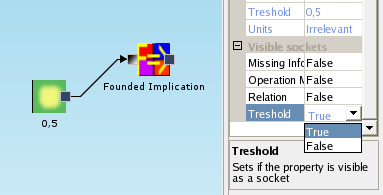
\includegraphics[width=7cm]{property_as_socket}
	\caption{A property as a socket}
	\label{fig:propertyAsASocket}
\end{figure}

Boxes can have also read-only properties. They are shown in the property grid, but they are not editable, their value is computed from current settings.

Each box module has a method which returns an object called \emph{functions}. This object represents the functionality of the box module. A box module has also an internal identifier, a label, an icon, a SVG design, names of categories, ``box modules asking for creation'', actions, a name of property driving label and a dynamic help.

\section{Ferda as a programming language}
\newtheorem{mydef}{Definition}

This section describes boxes as a function, formalizes boxes and introduces a new textual representation of connections between boxes.

The main concept of Ferda is to be user-oriented functional language. The basic abstraction is that a box is a function and sockets are properties of that function. There is no need to talk about properties, because properties are also accessible by sockets. It is a typed language. The box returns an object called \emph{functions}. A socket specifies which types of functions can be connected to the socket. A box also specifies which types of functions it returns. Types of functions are called ``Ice identifiers''. One object can have multiple such types.

Ferda is an environment for the language. We will call the language of Ferda the \emph{Ferda language}. The language has its syntax and semantics. The syntax is in Ferda about boxes and connections regardless their meanings. The syntax specifies how a connection can look like. The semantics of Ferda is specification how to compute a result of connection of boxes. Source codes of the Ferda language are connections of boxes. Source files of the language are project files of Ferda.

\subsection{Formalization of boxes}
Let us create a formalization of basic objects of the Ferda user-oriented language. It will not be used later in the text, but it will offer a more precise declaration of the language.

\begin{mydef}
\emph{Box} is an ordered pair $\left<S,F\right>$ where
\begin{itemize}
	\item $S$ is a set of sockets;
	\item $F$ is a set of functions which use sockets from $S$.
\end{itemize}
\end{mydef}

\begin{mydef}
\emph{Socket} is an ordered pair $\left<n,T\right>$ where
\begin{itemize}
	\item $n$ is socket name and
	\item $T$ is a set of box types.
\end{itemize}
\end{mydef}

Every functions object can have one or more \emph{Ice identifiers}.

\begin{mydef}
The \emph{$hasIdentifier(f,i)$} holds iff $f$ is function and $i$ is an Ice identifier of the function $f$.
\end{mydef}

\begin{mydef}
\emph{Box type} is an ordered pair $\left<i,S\right>$ where
\begin{itemize}
	\item $i$ is an Ice identifier;
	\item $S$ is a set of ordered pairs $\left<n,i\right>$ where
	\begin{itemize}
		\item $n$ is socket name;
		\item $i$ is an Ice identifier.
	\end{itemize}
\end{itemize}
\end{mydef}

\begin{mydef}
Box $B=\left<S,F\right>$ \emph{is of box type} $A=\left<i,Z\right>$ (we will shorten it as $isOfType(B,A)$) iff 
\begin{itemize}
	\item $(\forall \left<n,j\right>\in Z)(\exists \left<m,T\right>\in S)(\exists \left<y,W\right>\in T)(m=n \wedge j=y)$ and
	\item $(\exists f\in F)(hasIdentifier(f,i))$.
\end{itemize}
\end{mydef}

\begin{mydef}
A box $B=\left<S,F\right>$ \emph{can be connected} to a socket $s=\left<n,T\right>$ iff $(\exists t\in T)(isOfType(B,t))$
\end{mydef}

\subsection{Textual representation of the language}
\label{sec:formalisation}
A new textual representation of the Ferda language is described in this section. This representation is used in the next chapters. On many places screenshots of Ferda can be used as a presentation of functions, but you do not see every settings of the connections on them. For example you can not see properties of all boxes.

Because the Ferda language is a functional language the standard prefix notation was at hand. The problem is that parameters are in the standard notation in brackets divided only with commas. Identification of parameters is done by their order.

But parameters of sockets do not have any order. The only identification of them are their names. Hence we will prefix parameters with their names and the symbol of equality. Let us describe the notation.

If box $B$ has all its sockets unset (all properties have their default values) we will write such connection as
\begin{equation}
B()
\end{equation}

If box $B$ has some of its sockets set, but it is not important for us we will write such connection as
\begin{equation}
B(\dots)
\end{equation}

If box $B$ is connected to a socket with name ``socketName'' of box $C$ we will write such connection as
\begin{equation}
C(socketName=B())
\end{equation}

If box $B$ is connected to sockets with names ``socketName1'' and ``socketName2'' of box $C$ we will write such connection as
\begin{equation}
C(socketName1=B(), socketName2=B())
\end{equation}
or we can label a part of connection and reuse it in next connections, like
\begin{equation}
L=B(); C(socketName=L, socketName2=L)
\end{equation}
We will call in this text instances of boxes by a name of their type, for example $Table()$. If in the connection are more boxes of the same type we will distinguish them by subscript, for example $Table_1()$.

\section{Programmer's view of the Ferda system}
Programmers of the Ferda system need to have deeper knowledge than the users. This thesis talks about changes of internal parts of the Ferda system, hence we are going to describe the design of Ferda from the programmer's point of view.

Base parts of Ferda have been written in C\#~2.0. The Ferda runs on both .NET~Framework and Mono. Some modules use also the Java platform. The Ferda uses middleware Internet Communications Engine (\url{http://www.zeroc.com}) for a communication between its modules. Every module can be written in different language and run on different computer. For easier development, many third party libraries and applications are used---mainly NAnt (\url{http://nant.sourceforge.net}), NUnit (\url{http://www.nunit.org}), NDoc (\url{http://ndoc.sourceforge.net}), Netron Graphic Library (\url{http://www.orbifold.net/netron/}) and DockDotNet library (\url{http://sourceforge.net/projects/dockdotnet/}).

Ferda was released under second version of General Public License (\url{http://www.gnu.org/licenses/old-licenses/gpl-2.0.html}). It allows everybody to use it for free, redistribute it and change the code (providing the results are still under the General Public License).

The aim of the Ferda project was to create application which is internationalized, well documented, modular, user-friendly and conforms Microsoft standards in user experience.

\subsection{Architecture of the Ferda system}
\begin{figure}
	\noindent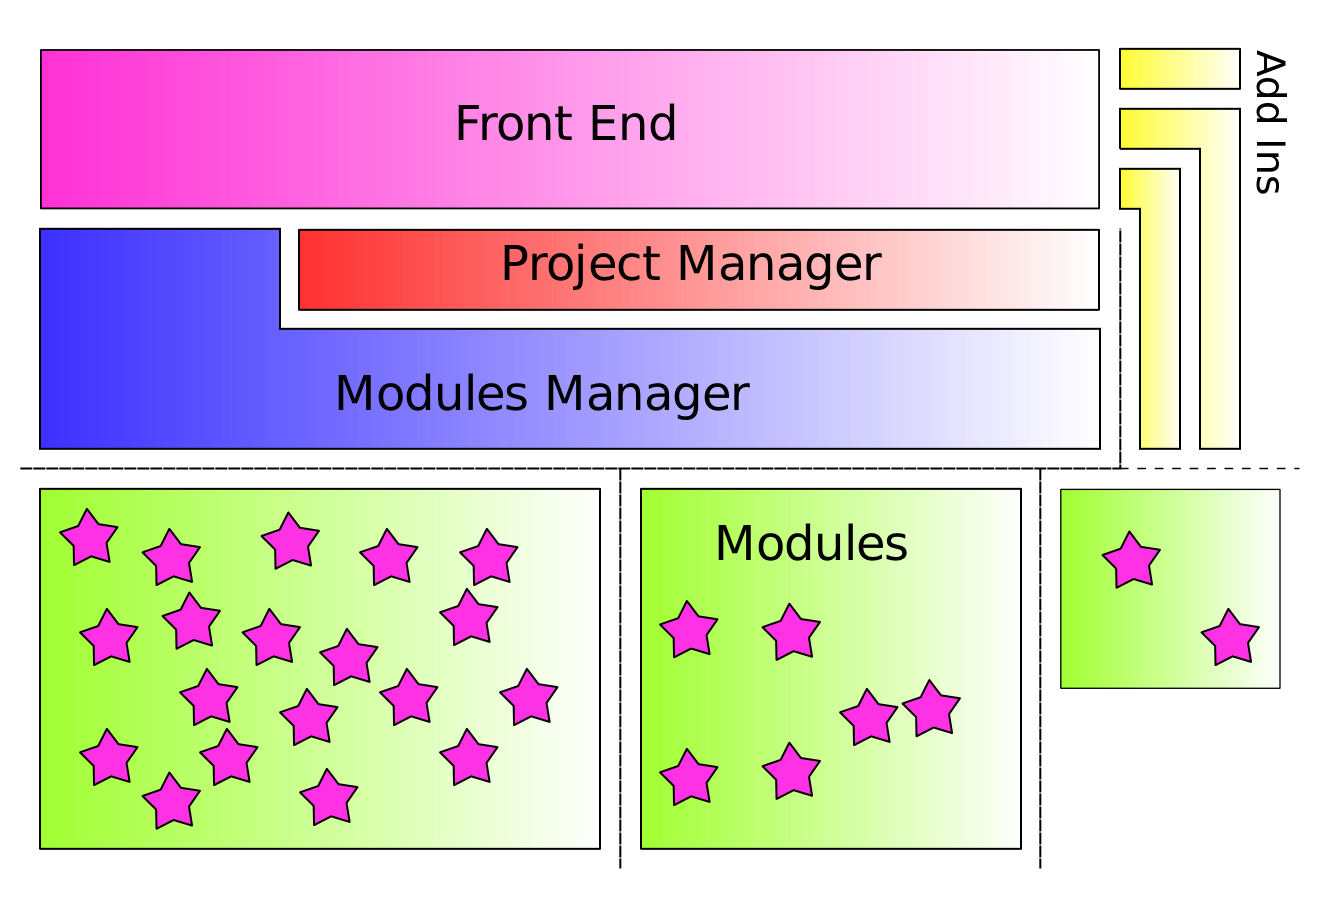
\includegraphics[width=1\textwidth]{designB}
	\caption{Architecture of the Ferda system}
	\label{fig:architectureFerda}
\end{figure}

Let us describe architecture of the Ferda system. Please see figure~\ref{fig:architectureFerda}. The main application is the FerdaFrontEnd.exe. It contains main visual parts of the Ferda system.

FrontEnd uses the assembly FerdaModulesManager.dll for communication with modules. This assembly is an abstraction layer so that FrontEnd does not know that modules are not implemented locally (it hides Internet Communications Engine).

Another assembly that is used by FrontEnd is the FerdaProjectManager.dll, which controls projects. This manager is able to load and save a project. Projects are stored in XML files.

FrontEnd also loads add-ins. Add-ins can extend functionality of FrontEnd in many ways. It is mainly used for modules for interaction and setting modules. Modules for interaction work on top of some box module. They for example show results of functions returned by the box module in user comprehensible way. Setting modules are used to help with setting nonstandard properties of boxes.

The communication between FrontEnd and modules and between modules themselves is via the Internet Communication Engine (Ice). Ice is a strong modern middleware. Thanks to Ice, Ferda is independent of both language and framework and it allows us to run different modules on different computers, without having a big computational overhead. It can be also used for distributed computing. Every Ice interface is defined in a special language called \emph{slice}. On figure~\ref{fig:architectureFerda} Ice is represented by the lines between squares.

IceGrid application, which manages available modules and loads them on demand, runs on a network. Modules manager uses these applications for getting modules. This application is part of Ice, hence on the figure it is also represented by the lines.

\subsection{Creation of new boxes}
This section of the thesis is not crucial for understanding the later parts of the text. It describes how modules create internally new instances of boxes. This part can be useful for a new programmer of boxes.  

Because of the use of Ice a creation of new boxes is more complicated. There is a need of distributed garbage collection. Please see figure~\ref{fig:creatorFactory}. Every box module implementation has its factory class. This factory class creates box module instances. There is one more layer---every box module factory has its factory class, we call it box module factory creator, which is a singleton.

\begin{figure}
	\noindent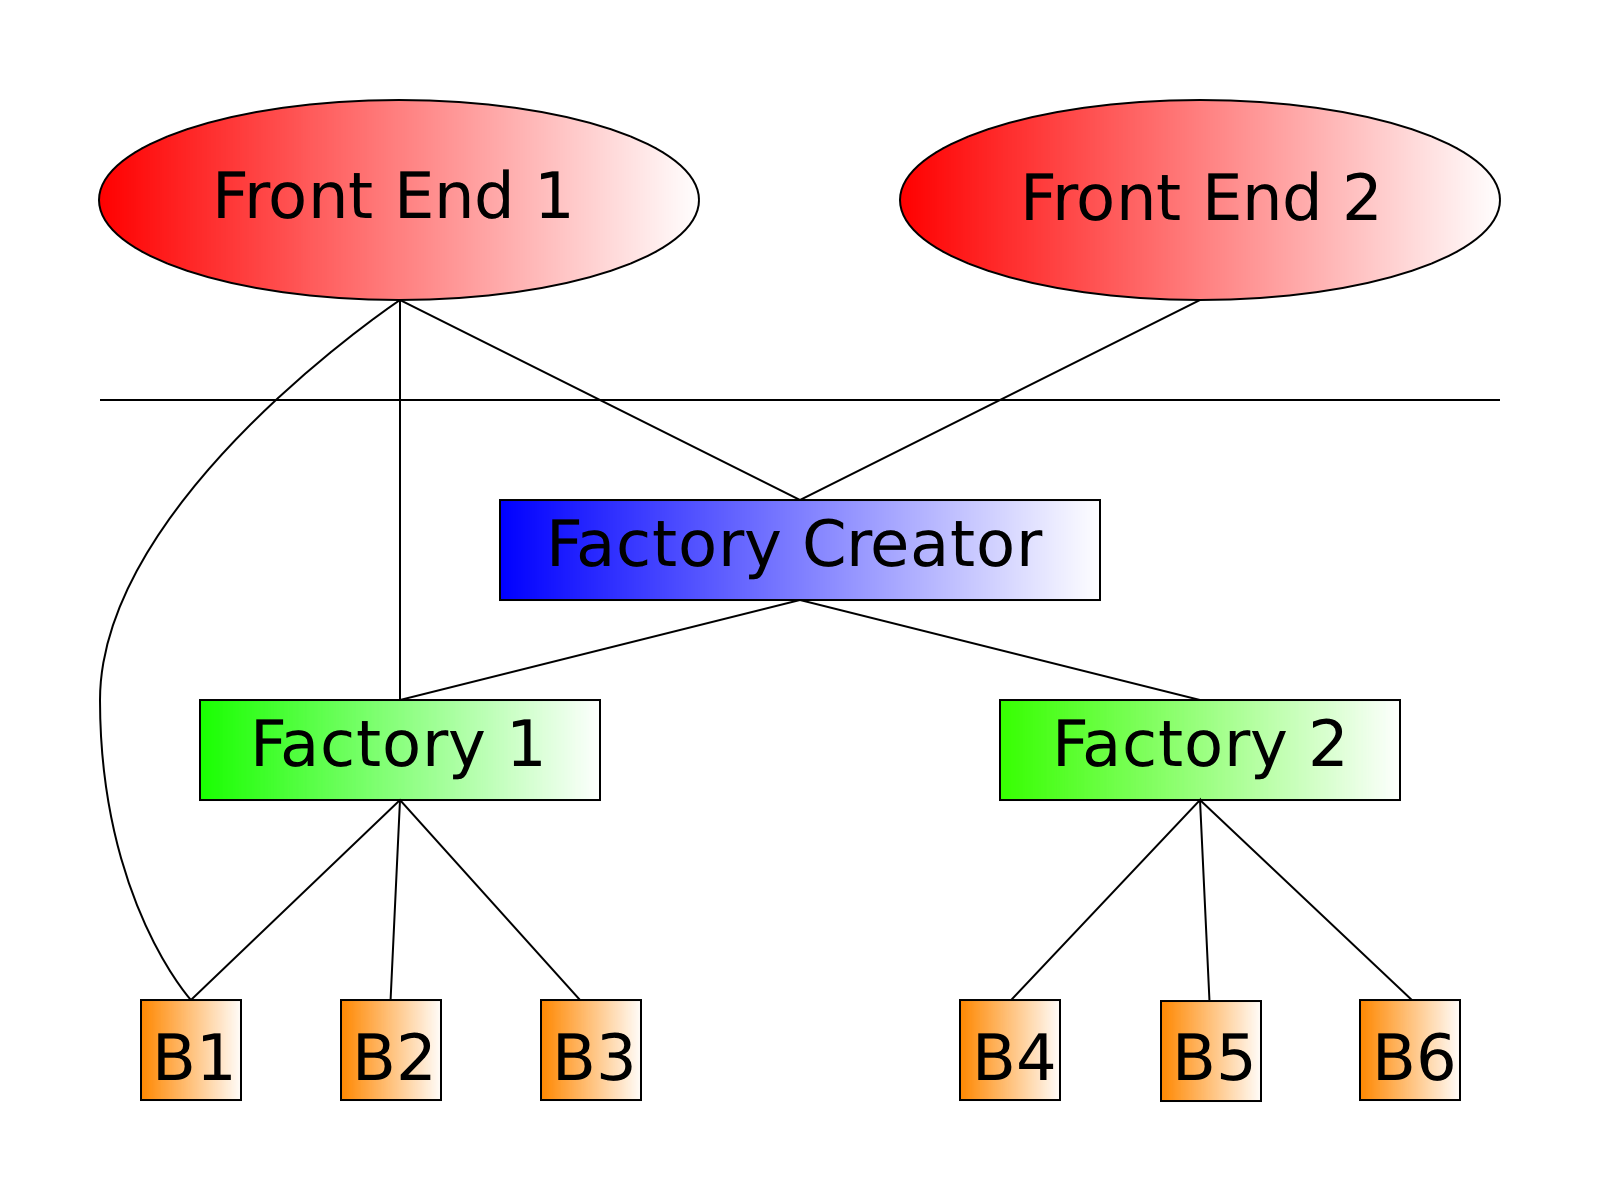
\includegraphics[width=1\textwidth]{creatorFactory}
	\caption{Creation of new boxes}
	\label{fig:creatorFactory}
\end{figure}

FrontEnd asks a box module factory creator for creation of only one box module factory for one box class. The creator has methods independent of both instance of the box module and FrontEnd connected. A factory has methods independent of box modules, but dependent on FrontEnd (for example localized names of properties). If FrontEnd is not connected for a longer time, all factory instances and box module instances are destroyed.

Word ``box'' in this thesis may mean two different things according to context---a box module or a box instance. A box module represents implementation. It has one instance of Ice box module factory creator interface which is registered in a IceGrid. A box instance is an instance of Ice box module interface. One box module can have more box instances.

\chapter{New features for visual programming}
This chapter describes the Ferda system as a visual programming language. It presents possible objects of the language and tools and utilities for the programming.

First, the thesis focuses on source codes of the language, because it is better to begin with syntax of a language than with its semantic. The section identifies one particular problem of projects of the Ferda system, it is the reusability of written code, and it describes several possible solutions. One particular solution is implemented as part of this thesis.

Subsequently, the thesis deals with details of the basics of visual functional programming. It explains why the language was chosen as functional and describes properties of functional languages.

The crucial part of this chapter is a set of proposed new boxes. These represent basic functions for the language. Some of them are implemented as part of this thesis. The new boxes have been chosen so that they brings basic functionality which other languages have. The boxes were also designed in mind of possible usage with data mining boxes. Several problems of data mining were in mind when we were thinking about the new boxes. But these problems are not remarked in this chapter, because the proposed boxes are generalized for being used by other applications.

The last part of this chapter describes advanced possible topics of the language. It proposes unit tests in the Ferda language and distributed computation in the language.

\section{Source codes and reusability}
\label{sec:reusability}
Every programming language has its own ways how to reuse code. This part of thesis is about ways how to make a programming in Ferda efficient. The need of rewriting a code and lack of user specified structure in boxes could result in a usability problem of any language in Ferda. Several ways how to solve these problems are shown and one implementation of such solution is described.

\subsection{Project import}
The simplest way is to copy the source code to different place and use it for different project. The same is possible in Ferda, you can copy a project file and reuse it.

With standard textual source code it is easy to merge the code from more sources. You can do it with the Ferda project, but you must merge a code in a project files manually in a text editor. The merging is not an easy process, thus it is not so much user-friendly way.

It would be convenient to have a functionality in Ferda that would allow us to import some or all boxes from one project into another. One way to achieve that would be adding a new item ``import project…'' to the Ferda menu. Therefore, if a user selected this item, a dialog for choosing project file would open. Having selected a project, the dialog with boxes in selected project should be shown. The user could select boxes which he would want to import. The last step would be the actual import of selected boxes.

Let us discuss the dialog box where a user could select boxes. To choose whole functions, seeing the dependency among boxes would be crucial. However, should the user selects to import a box without a box connected to this box, the box would be imported, but the result of such box could differ significantly from the situation before. On the other hand, such choice could be purposeful should the user want to connect to that box some box from the original project.

\subsection{Project using}
The source code of one application is usually not placed only in one source file, but in several. There are more ways in programming languages how to achieve this. One way typical for compiled languages is compilation of application from more source files from the beginning. A compiler has a set of files as an argument. The other way, specific for interpreted languages, is an import of another files into the source file. An advantage of this approach is that the imported file is loaded when it is used---hence the file can be created a short time before usage. It allows us to write code which loads every file in some directory and hence it can be used for plug-ins. Even compiled applications have a way how to achieve this functionality. Compiled applications can use libraries (or assemblies or modules) which can be loaded dynamically on demand. It can be also used for loading a source file on demand if a compiler for that language is available on machine where the application is being executed.

If we wanted to add this to Ferda, project would have to have a new attribute defining the using of other projects. Boxes from such projects would have to be read only---no change of properties and boxes connected to their sockets would be available. Also, the origin of each box should be clearly traceable.

Nevertheless, the import itself of projects into other projects presents a demanding situation. Let us illustrate this on the following example: let us have two imaginary projects, $A$ and $B$, with corresponding boxes, $A$ and $B$. The project $B$ is imported by the project $A$, and the box $B$ is connected to the box $A$ in the project $A$. Even if we remove the box $B$ in the project $B$, maintaining the information about the former connection to already non-existent box $B$ in the project $A$ would facilitate the reversible operation in case we needed to add the box $B$ back into the project $B$. This would allow us to change boxes and therefore functionalities.

Let us discuss possible implementation of such imports. Information about imported projects should be serialized to a project files. In the project file there should be a section with paths of imported project files. Boxes which are used from other projects should not be serialized, but connections of these boxes in the project and their position on desktops should. It raises a question how to identify these boxes. The first solution which comes into consideration is to use as identification a pair of a project identifier of a box and an identifier of an imported project. Such solution would have problems which should be resolved.

At this time boxes are identified in one project by project identifier. The project identifier is an integer which grows from one up without the awareness of the user. If the user removed a box with the last project identifier, exited Ferda, started Ferda, reopened the project and added a new box, the new box would have the same project identifier as the removed box had. If we still liked to use the project identifier as identification of boxes we should avoid this by serializing the last used project identifier in the project. To be able to replace a box, it is vital the user be able to choose the project identifier.

%tady by mohlo byt jak by melo vypadat menu a ze maji byt videt importovane veci v archivu
\subsection{Network archive}
Another way how to reuse a box can be to copy it from another project. Let us have a new place where you can place boxes which you want to reuse. Such place can be on network and more users can place their boxes there and reuse them in other projects. They can use such place to move their work to others. Let us call this place a network archive.

\subsubsection{Implementation}
As part of this thesis, the present author has created a simple implementation of such network archive. The main part is a Ice service which is running somewhere on network. It has simple definition in slice:
\begin{verbatim}
interface Archive {
	/**
	 *
	 * Adds a box with connected subboxes to the archive
	 *
	 **/
	void addBox(Box boxValue, string label)
		throws NullParamError, NameExistsError;

	/**
	 *
	 * Removes the box from archive
	 *
	 **/
	void removeBox(string label)
		throws NameNotExistsError;

	/**
	 *
	 * Gets box which is in the archive
	 *
	 **/
	Box getBox(string label)
		throws NameNotExistsError;

	/**
	 *
	 * Gets labels of boxes in the archive
	 *
	 **/
	idempotent Ferda::Modules::StringSeq listLabels();
};
\end{verbatim}

The Network archive is a collection of boxes (with all their sub-boxes---boxes connected both directly and indirectly to that box). Each box is identified with some label. You can add a box and remove a box, get information about a box and list all labels in the collection. The collection is serialized on a disk every time it changes. After startup of the service, it loads the last serialized version.

From the user perspective the network archive is a new panel with list where you can copy a box to. Please see figure~\ref{fig:addToNA}. 
\begin{figure}
	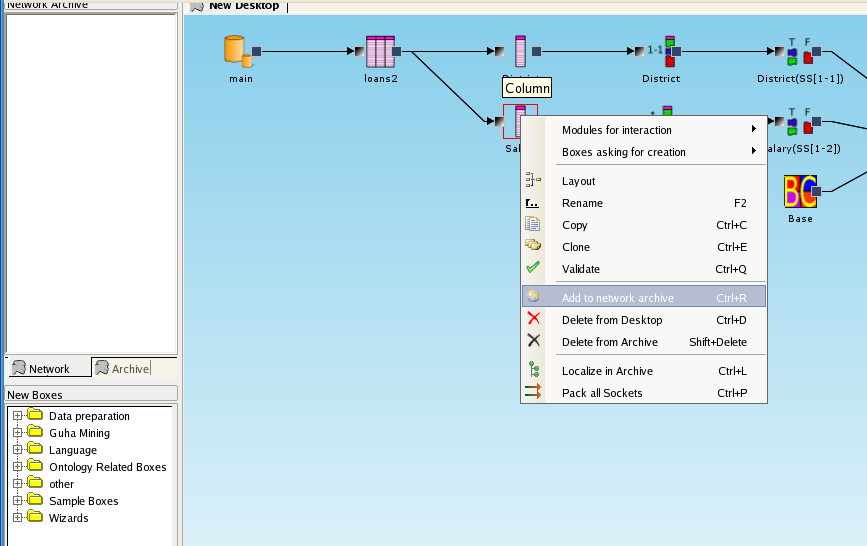
\includegraphics[width=1\textwidth]{add_to_network_archive}
	\caption{Add a connection to the network archive}
	\label{fig:addToNA}
\end{figure}

It will ask the user to enter a label after dragging a box from desktop to the network archive. Please see figure~\ref{fig:setNameInNA}.
\begin{figure}
	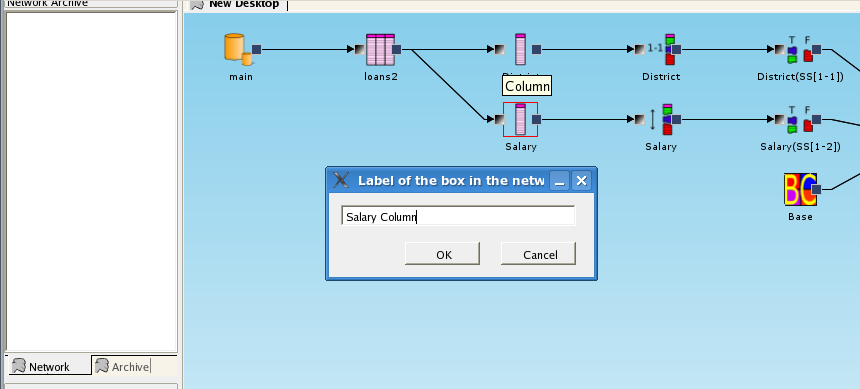
\includegraphics[width=1\textwidth]{set_name_of_box_in_network_archive}
	\caption{Set a name of box in the network archive}
	\label{fig:setNameInNA}
\end{figure}

After that a new item with selected label should be visible in the list. Please see figure~\ref{fig:addedToNA}.
\begin{figure}
	\centering
	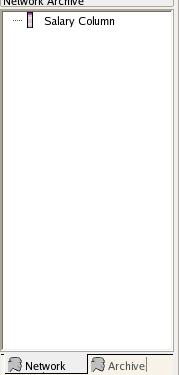
\includegraphics[height=7cm]{network_archive_box_added}
	\caption{New box added to the network archive}
	\label{fig:addedToNA}
\end{figure}

The user can then go to another computer which uses the same network archive and drag the box from network archive to another project. It should create a new copy of the box with all its sub-boxes on the desktop. Please see figure~\ref{fig:dragFromNAToDesktop}.
\begin{figure}
	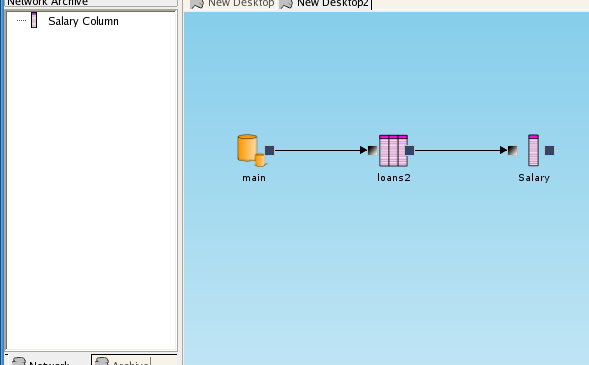
\includegraphics[width=1\textwidth]{network_archive_drop_to_desktop}
	\caption{Drop box to a desktop from the network archive}
	\label{fig:dragFromNAToDesktop}
\end{figure}

They can also remove the box from the network archive. Please see figure~\ref{fig:removeFromNA}.
\begin{figure}
	\centering
	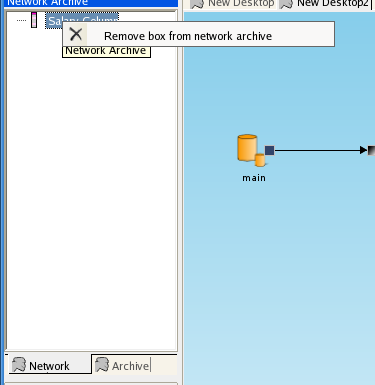
\includegraphics[height=7cm]{network_archive_remove_box}
	\caption{Remove box from the network archive}
	\label{fig:removeFromNA}
\end{figure}

\subsubsection{Future enhancements}
Organizing boxes in network archives into some structure would facilitate the work. It could be an one-level structure (labels) or a tree-structure like in directories. Another enhancement would be to add user rights to these labels.

Easy thing to do is to allow the Ferda FrontEnd to work with more network archives.

\section{Functional visual programming}
We have decided in Ferda that boxes represent functions and the language of Ferda system is functional. Many visual programming languages exist, but we do not know about any which is functional. Most of these languages are dataflow, workflow or object-oriented languages. The biggest difference between these languages and a functional language is that in a functional language a result of program is a return value of some function.

The result of functional programs are counted by the evaluation of mathematic functions. Pure functional programming does not work with states and mutual data.

In a visual programming language it means that the execution of a program is a tree of boxes where root of the tree is an endpoint of the execution. The tree is similar to the connection of the boxes on a desktop, only cycles are expanded and two uses of the same box are in the execution two independend boxes. In workflow and dataflow languages there can be more endpoints. In the object-oriented languages there is one main object which is responsible for the execution, but from the connection of boxes it is not possible to know the execution plan. It works with mutual data.

When Ferda was being designed we took a look on other two data-mining tools---Weka (\url{http://www.cs.waikato.ac.nz/ml/weka/}) and Clementine (\url{http://www.spss.com/clementine/}). The first is open sourced the second is commercial. Both Weka and Clementine offer workflow visual programming languages.

We are able to naturally represent objects of interest with a functional language. Ferda has typically more boxes for the same task than some workflow oriented visual programming language. Workflow and dataflow oriented languages have more settings in a property grid and dialog boxes. So we can say that the language of Ferda is more low leveled.

Several reasons guided authors of Ferda to make the language in Ferda functional. GUHA~\cite{GUHAbook} is a theory which has its own logical calculus. Formulas of any calculus are mostly represented like functions. The semantics of formulas can be seen as a value of the functions. It means that a calculus can be viewed as a functional language. Big similarity between functions and formulas can be also found in constructions of transparent intensional logic (\url{http://til.phil.muni.cz}). Both have as a base the typed lambda calculus. Functional language is in many ways close to the natural language. 

LISp-Miner has mostly for each type of GUHA method three programs---the first for setting of the task, the second for generating results and the third for browsing the results. The partitioning has been affected by work flow of data mining. If we had done Ferda workflow oriented, it would have three boxes for one task which would correspond to the three programs of LISp-Miner. Ferda has advantage of reusability compared to LISp-Miner, because setting of a task is done by many boxes. It would not have if we had done Ferda workflow oriented. 

Functional languages are typically full featured scripting languages. They are part of many scientific applications, because writing in such languages is similar to classic mathematical functions used in scientific texts. Thus scientists used to use such languages. Workflow and dataflow languages are typical for concrete problems. The set of rich boxes for the specific problems are prepared in such languages. Typically they are strong at the things they were designed for, but it is hard to use them by a user for something else.

This thesis brings some new boxes, which are described in the section~\ref{sectionNewBoxes}. Ferda is full featured language thanks to these boxes. It means that it can be used for most computer tasks. The language is recursively enumerable.

\section{Language boxes and expressions}
\label{sectionNewBoxes}
Every programming language has from the beginning at least a small set of functions. Also it has some way how to use these functions to create more complex ones. Such an instrument has been created for Ferda as a crucial part of this diploma thesis. New language boxes are presented at this part of thesis. Data-mining examples which use these boxes are shown in chapter~\ref{chap:KDDExamples}.

\subsection{Constants}
The Ferda language is a typed language. It means that functions in Ferda return values of some type. Easiest functions are constant functions which return specified value. There are at least two ways how to achieve this by box semantic. One way is to create a specific box type for each type of constants which returns that specific type. This type has been created in Ferda as a part of this thesis.

!-- TODO přidat obrázek --!

The other way is to create one box type which has one property for specifying a type and dependent on it it would have a second property with a value of a specified type. It would return that value.

\subsection{Boxes for mathematics}
Mathematical expressions are really necessary for programmers, statisticians and analysts. Support for them is important. Boxes for basic mathematical functions have been added.

\subsubsection{Binary operation}
Binary operation box has been implemented as part of this thesis. It has three properties. First two, called ``value1'' and ``value2'', are arguments of an operation. Their type is double. The last property is the operation sign ($+$, $-$, $*$, $/$), it is called simply ``type''. Result of such operation is always double. Please see figure~\ref{fig:boxBinaryOperation}. In the figure you can see that ``value1'' and ``value2'' properties are set by sockets.
\begin{figure}
	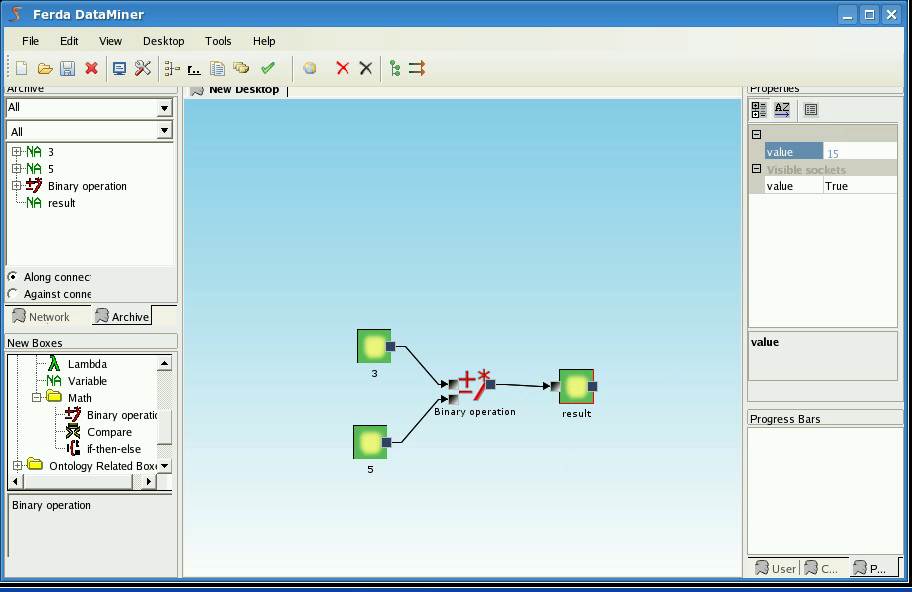
\includegraphics[width=1\textwidth]{binaryOperation2.png}
	\caption{Binary operation}
	\label{fig:boxBinaryOperation}
\end{figure}

Such box can not be used for setting up integer properties, even if it sums only integers, because it always returns double. One way how to overcome such problem is to introduce a new convert box. The second way is to change the behavior of the binary operation box. It would return an integer if it summed two integers. Similarly it would return a float if it summed an integer with a float or two floats. Different operation types would behave differently as it is standard in other languages. Such function would be less efficient, but more useful.  

There is no need to have one box for all operations. There can be also as many boxes as many operations are. Let us describe how to create for example a plus box. There are more possibilities how to do it. It has been already described in~\cite{znalosti2006} on a plus box. There could be a plus box which would have two properties ``value1'' and ``value2'' like the binary operation box. But there could be also a plus box which would have only one socket ``arguments''---the box would sum all boxes connected to this socket. It means less boxes on the desktop when summing more numbers. Also it adds an easy way how to sum sequences of numbers which are described in section~\ref{sec:sequences}. But even without such box we are able to do it (for example thanks to head/tail box which is described in the same section), only it is more complicated.    

\subsubsection{Comparison}
Comparison functions are functions of two arguments which return a boolean value. As part of this thesis a compare box has been created which has three arguments. First argument is the type of the comparison function, next two arguments are doubles. This box has implemented basic mathematic comparisons ($<$, $>$, $<=$, $>=$, $=$, $!=$). Please see figure~\ref{fig:boxCompare}.
\begin{figure}
	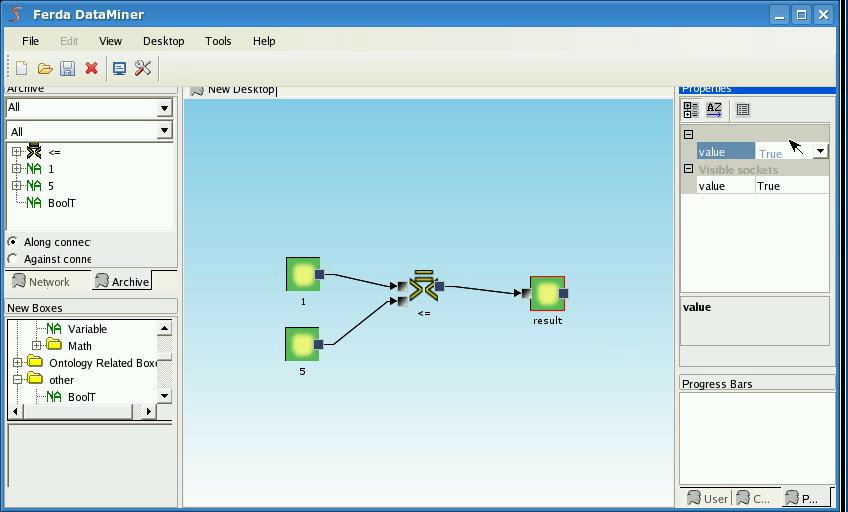
\includegraphics[width=1\textwidth]{compare2.png}
	\caption{Compare}
	\label{fig:boxCompare}
\end{figure}

It is possible to create also boxes specific for every comparison function like has been described for the binary operation box.

\subsubsection{If expressions}
If expression is a function which has three arguments. The first argument, called ``if'', is of boolean type. The expression returns value of the second argument, called ``then'', if the first is true, otherwise it returns the value of the third argument, called ``else''. Such new box, called ``IfThenElse'' has been created. Please see figure~\ref{fig:boxIfThenElse}.
\begin{figure}
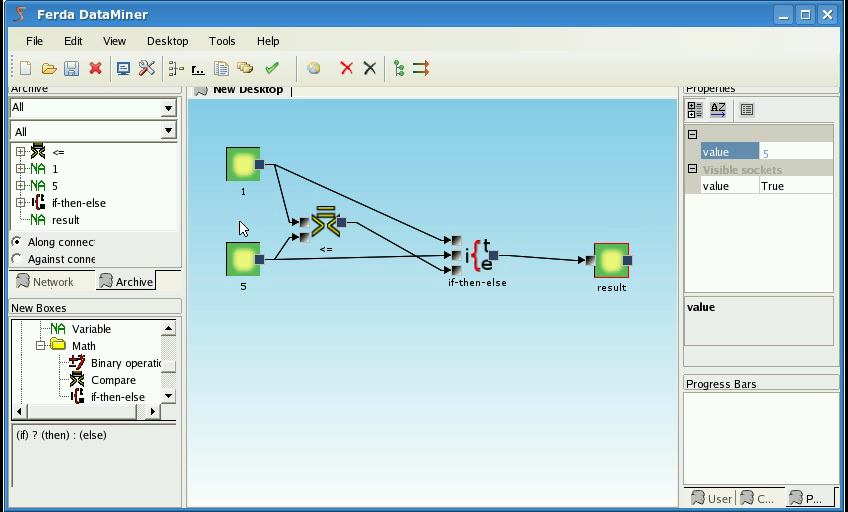
\includegraphics[width=1\textwidth]{ifthenelse2.png}
	\caption{If expression}
	\label{fig:boxIfThenElse}
\end{figure}

Important fact is that if the ``if'' argument were true, the function in the ``else'' socket would not be computed. Similarly, if the ``if'' argument were false, the function in the ``then'' socket would not be computed.

\subsection{Lambda expression}
Lambda is one of the most important expressions for functional languages. Its base is in the lambda calculus. Mathematicians define many times define functions for later use. For example see definition of this ``plus one'' function
\begin{eqnarray*}
f(x)&=&1 + x\\
y&=&f(9)
\end{eqnarray*}

This equations gives to the $y$ value $10$. In the lambda calculus it equals to this expression
\begin{eqnarray*}
f&=&\lambda x.(1+x)\\
y&=&f(9)
\end{eqnarray*}

The naming of functions is not necessary, it can be also written as 
\begin{eqnarray*}
y&=&(\lambda x.(1+x))(9)
\end{eqnarray*}

Lambda can be seen as a function which has two arguments---the first argument is a set of variables and the second argument is a expression which uses these variables. It returns a function from the variables to the value of the expression after setting up the variables.

Mathematicians can also define recursive functions like factorial
\begin{eqnarray*}
f(0)&=&1\\
f(x)&=&x * f(x - 1)
\end{eqnarray*}

The same thing can be done in functional languages with lambda expression. The ``plus one'' function will be presented now in more languages with use of lambda expression. However let us show the first example not on a functional language but on a imperative one with functional aspects. Such language is the C\# 3. Lambda expression is in the C\# 3 done by operator $=>$:

\begin{verbatim}
public delegate int function(int x);

public static void Main(string[] args)
{
  function plusOne = x => 1 + x;
  var a = plusOne(9);
  System.Console.WriteLine(a);
}
\end{verbatim}

F\# is another language which is translated to IL of .NET framework, but it is a functional language. The lambda expression is done by the \emph{let} operator there:
\begin{verbatim}
let onePlus x = 1 + x
do printf "%s" (onePlus(9)) 
\end{verbatim}

The last example is written in a more commonly used language today, in Python. It is a object-oriented scripting language with both imperative and functional aspects. There is used the \emph{lambda} keyword:
\begin{verbatim}
plusOne = lambda x: 1 + x
print plusOne(9)
\end{verbatim}

A new lambda box has been created as part of this thesis. It has a socket ``Function'' and a property ``VariablesCount''. Type of this property is integer. There are as many socket pairs (variable, value) as big the value of this property is. It is the first box in Ferda which has dynamic sockets. Such thing has been designed in the beginning of Ferda, but because it have not been used, some changes were needed to the core of Ferda to make it running.

Please see figure~\ref{fig:boxLambdaBasic}. The ``Function'' socket represents the expression from the lambda. The ``VariablesCount'' is set to zero in this connection. It means that the lambda returns the same thing that is connected to the ``Function'' socket. In this example the result is 6, represented as double. 
\begin{figure}
	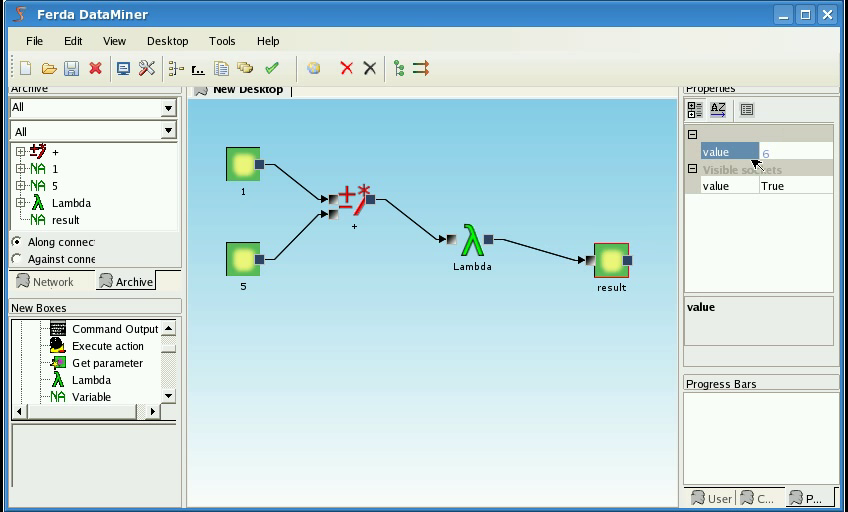
\includegraphics[width=1\textwidth]{lambdaBasic2.png}
	\caption{Lambda without arguments}
	\label{fig:boxLambdaBasic}
\end{figure}

Please see figure~\ref{fig:boxLambdaOnePlus}. It shows the same example in Ferda as we have seen in the previous examples in other languages---the one plus function. The ``VariablesCount'' is set to 1 in this connection. It means there are sockets ``Variable0'' and ``Value0''. The box with value 5 is used there as a variable. The box with value 9 is the value of variable. Hence, the result of such connection should be 10.
\begin{figure}
	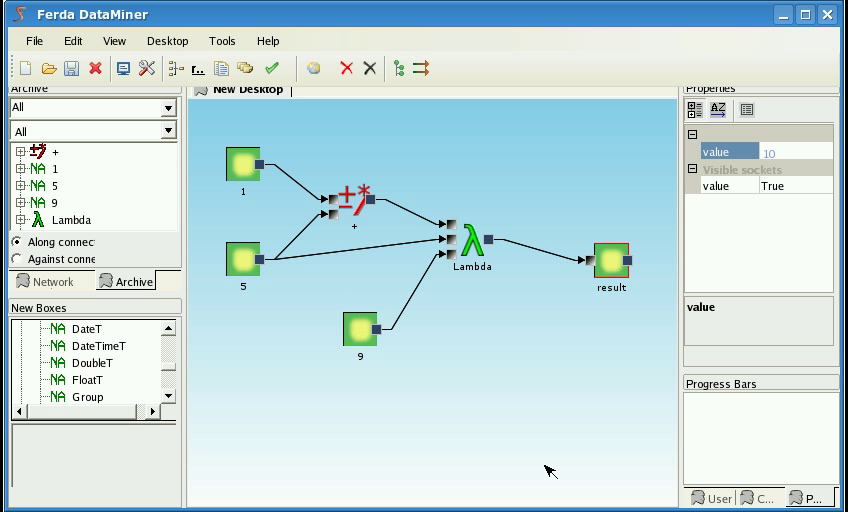
\includegraphics[width=1\textwidth]{lambdaBasic3.png}
	\caption{Lambda with one constant parameter specified}
	\label{fig:boxLambdaOnePlus}
\end{figure}

The type of boxes which can be connected to the ``Value0'' socket are determined by the types of box which is connected to the ``Variable0'' socket. Multiple boxes can be connected to the ``Variable0'' socket. The determined type is then the intersection of the types of those boxes.

It is possible to use as a variable not only a variable box, which has not been introduced yet, but any kind of box. Moreover, this box has other boxes connected to it, which enables a simple representation of recursive functions. This is described in latter parts.

\subsubsection{Implementation of the lambda box}
If the lambda box is asked for its functions object it will clone the connection which is in the ``Function'' socket, only instead of boxes which are connected to some variable socket it places a cloned connection to value socket of that variable there. The lambda box returns the functions object of the main box from the cloned connection.

The cloning is not done in the lambda box, but the project manager is used. Its interface has been extended for cloning functionality as part of this thesis.

In the lambda calculus it is possible that the variable is a non-constant function. For example:
\begin{equation}
\lambda x.(1+x(5))(\lambda y.(1+y))
\end{equation}

This is not possible within the implementation in Ferda, because the implementation replaces variables with cloned values without reconnecting to the cloned value connections of the variable. Such thing can be implemented, however, there are several complications which must be overcome. One of these is that the lambda box should be able to name its value sockets. Hence, it is possible to create a lambda box with the same box type as any other box has.

The implementation has one problem, which is not easy to fix. The cloned boxes are not released until the end of the FrontEnd application even if they are not used and every time any box asks for functions object of the lambda, new cloned boxes are created. It means that the total amount of used memory raises when the lambda box is used. It is not easy to fix, because there is no information when a box leases to use a functions object. Adding such information to Ferda would require changes to almost all boxes.

There is also one performance problem. Let us have function $\lambda x.(x*x)$. In most of functional languages, if you called such function with parameter $1+1$, it would firstly compute $1+1=2$, and later it would pass 2 as the $x$---hence it would compute $2*2$. In Ferda such function created by a lambda box computes $(1+1)*(1+1)$. It means the plus operation is computed twice. This problem grows when the lambda box is used for a recursion. A generic fix is problematic, because in Ferda there are functions which can not be stored in a simple class and the connection to other boxes is necessary. For simple types some cashing mechanism can be created.

\subsubsection{Example usage of lambda: the factorial}
Let us take a look at how the lambda can be used for a recursive function. One of the simplest recursive function is the factorial. Simple imperative version of that function in the C\# language is: 
\begin{verbatim}
public static int Factorial(int x)
{
  if (x == 0)
  {
    return 1;
  }
  else
  {
    return x * Factorial(x - 1);
  }
}
\end{verbatim}
	
A better implementation of the factorial in C\# could use the \emph{if expression}:
\begin{verbatim}
public static int Factorial2(int x)
{
  return (x == 0) ? 1 : x * Factorial2(x - 1);
}
\end{verbatim}

The factorial in Python can be implemented this way:
\begin{verbatim}
fac = lambda x: x == 0 and 1 or x * fac(x - 1)
\end{verbatim}

And the last implementation is in F\#:
\begin{verbatim}
let rec factorial n =
    if n=0 then 1 else n * factorial(n - 1)
\end{verbatim}

Please see figure~\ref{fig:factorial}. This figure shows the implementation of the factorial function in Ferda.
\begin{figure}
	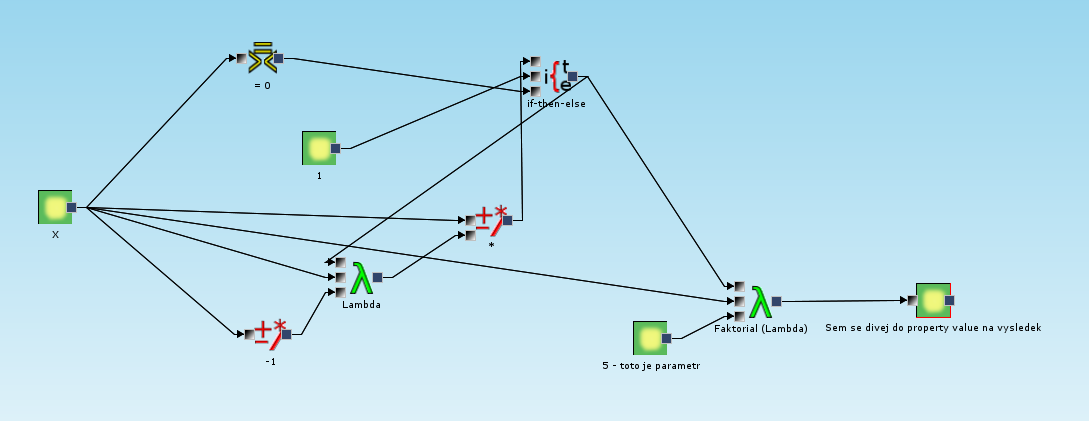
\includegraphics[width=1\textwidth]{faktorial}
	\caption{Factorial}
	\label{fig:factorial}
\end{figure}

When you are working with the lambda box in a recursion you should be aware of interminable functions. For example if a user clicked on a plus box in the center of figure~\ref{fig:factorial}, the program would compute infinitely, because the plus box has read-only property ``value'' and it should be set to $factorial(-1)$ computed by the connection in the figure. An easy fix for this problem is to replace the condition $x=0$ with a condition $x<=0$. Since it is easy to create an interminable function and execute it, it is preferable to save the project file very often.

\subsection{Sequences and sets}
\label{sec:sequences}
It is possible to represent a sequence of numbers by numbers only using basic primary recursive functions. But if there is a need of easy computable sequences of function it is better to add a support for that to the language.

The Ferda includes a box called Group. This box is the only box which is not a real back-end module. It is implemented in the modules manager. It has one socket and the box represents all boxes which are connected to this socket. If second group box is connected to the first one, the first box represents all boxes which are connected to the first box without the second group box but with all boxes which are represented by the second group box. If the box is connected to a socket to which it is possible to connect more boxes, it means that all boxes which are represented by the box are in the socket. The group box is very useful for organization of boxes on the desktop and reuse of a set of boxes.

We want to have a possibility to create a box which would represent a sequence of boxes like the group box, but the box should be a standard back-end module. The box should return as a value a sequence of functions classes instead of one functions class. Thus we need second-order functions. It is an easy thing in Ferda---define a functions object for sequence which has methods which return members of the sequence---functions objects. Then a sequence box can be created. There are more ways how to create a sequence in the language. For example one way is to have a box with property called ``count of items'' and when it is set to some number that number of sockets will appear. These sockets represent items of a sequence. Another boxes can be ``head--tail'' box (Lisp and Prolog use such ``functions''), ``clear sequence'',  ``add an item to the end'', etc. Also standard high-order functions for working with sequences in functional languages would be useful (the map, fold and filter functions)~\cite{webHighOrderFunctions}. The map function is described in the next section.

If a socket has an ability to connect more boxes, we might want a way to connect all functions in some sequence to that socket. The implementation of connecting a box to a socket could be changed for that. A new implementation could first try if the functions object is a sequence functions object. If it were true, it would connect the functions objects inside the sequence, otherwise the functions object itself.

The main implementation of a box module has a method which is used for determining which functions are connected to a specified socket. It has this signature:
\begin{verbatim}
public ObjectPrx[] GetFunctions(string socketName)
\end{verbatim}

The implementation of this method could be changed so that if it is possible to connect more boxes to socket ``socketName'', first try if the functions connected to that socket is a sequence. If it is true, do not return the sequence object, but all functions which are in the sequence. Otherwise the implementation should return the same result as the original implementation.

Such change would give us the ability to use sequence boxes as a group box.

\subsubsection{Map box}
It could be very useful to have a box which would enable us an ability to transform a sequence into sequence the way that for each item in the sequence the same function would be used. For example we would like to have a possibility to create from a sequence of numbers a sequence of their squares. 

We are going to call that new box ``Map''. It would have three sockets ``What'', ``Do'' and ``Variable''. The incoming sequence should be connected to the ``What'' socket, the function which changes the items should be connected to the ``Do'' socket and the function should use a variable which should be connected to the ``Variable'' socket. The variable would be replaced by the items in the incoming sequence. The result is a sequence of cloned functions where the variables were replaced by items in the incoming sequence.

The previous example with squares could be implemented this way:
\begin{eqnarray*}
Map(&&What=Sequence(I1=1,I2=2,I3=3,I4=4), \\&& Do=Operation(Type="*", Value1=X, Value2=X), \\&& Variable=X)
\end{eqnarray*}

The Map box is just a specific implementation of a standard function in the functional programming. However, there is a small difference compared to other languages. The difference is in the existence of the ``Variable'' socket. In standard languages the function has two parameters: a function (our ``Do'' socket) and a sequence (our ``What'' socket). Because parameters of functions are sorted in standard languages, some convention can be used for the variable. For example the variable can be the first parameter of the ``Do'' function. Nevertheless, we have not proposed such way, because parameters are not sorted in Ferda.

\subsection{Other new boxes}
\subsubsection{Get parameter}
Boxes can have read-only properties. They are shown in the property grid, but they are not editable, they are computed instead. These properties can be seen as another output of a function which a box represents. If we wanted to use such result by different boxes, we would need a way how to get a value of a read-only property. Such way is the new GetPameter box which has been implemented as a part of this thesis. Please see figure~\ref{fig:boxGetParameter}.

\begin{figure}
	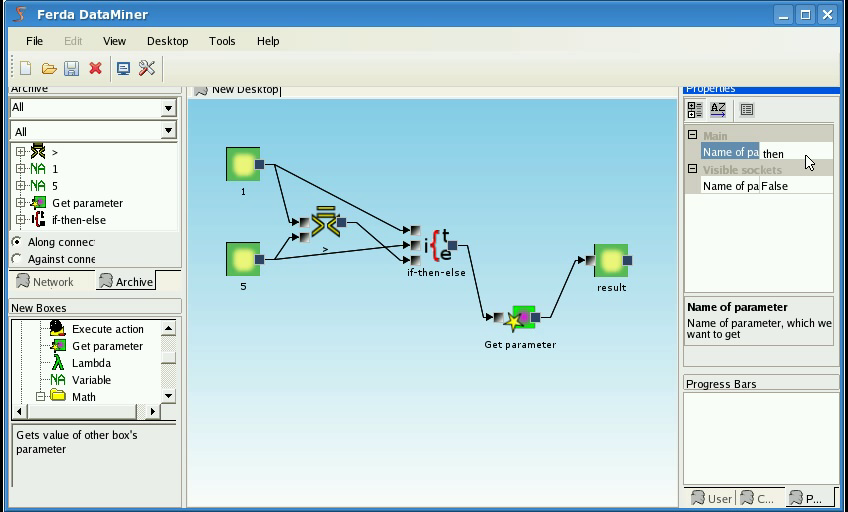
\includegraphics[width=1\textwidth]{getParameter2.png}
	\caption{Get parameter}
	\label{fig:boxGetParameter}
\end{figure}

The box can get values of properties of any box even of properties which are not read-only. It can also get functions objects of boxes connected to sockets of any box. The word ``Parameter'' in the name of the box means parameter of function which the box represents. Parameters can be set by a property or by a connection to a socket. The GetParameter box has a property named ``ParameterName'' and a socket named ``Box''. The socket specifies a box of which parameter we are interested in and the ``ParameterName'' is a name of a socket or a property we are interested in.

\subsubsection{Execute action}
A box can have actions. These actions could be executed separately by a user of the Ferda system in FrontEnd. There were not possibility of executing such actions as part of a program in the Ferda language. That is why a new box called ``ExecuteAction'' has been created as part of this thesis.

Please see figure~\ref{fig:boxExecuteAction}. ExecuteAction box has one property called ``ActionName'' which specifies name of action which should be called. It has also two sockets. The first is called ``Box'' and is for specifying a box whose action should be called. The second is called ``Function'' and serves for specifying the box which is used for getting the functions object.

When the ExecuteAction box is asked for a functions object, it executes action of a box in socket ``Box''. After that it returns functions object of a box in socket ``Function''.

\begin{figure}
	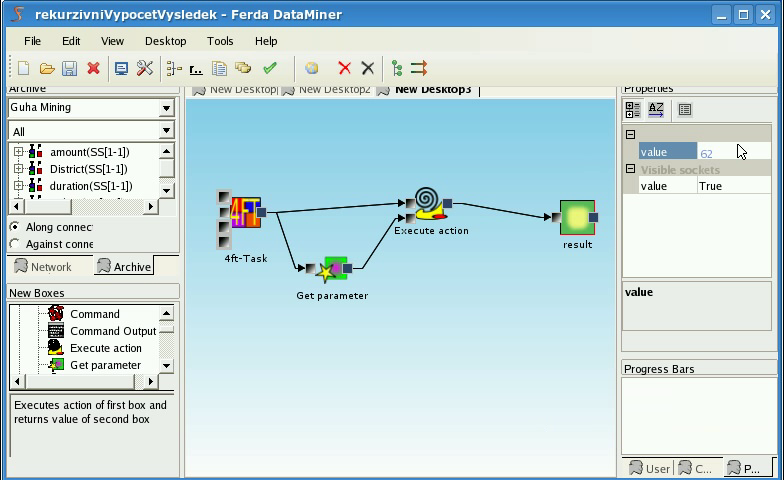
\includegraphics[width=1\textwidth]{executeAction2.png}
	\caption{Execute action}
	\label{fig:boxExecuteAction}
\end{figure}

Actions belong to the paradigm of imperative programming and the ExecuteAction box is a way how to translate actions to the functional language. 

\subsubsection{Command and command output}
It can be useful to have a possibility to execute external application and read output of that application. Two new boxes have been implemented as part of this thesis for this purpose.

The first one can execute a command, and is called ``Command''. More these boxes can be connected together. Output of one command is then used as input of the next command.

The second box which has been created is called ``CommandOutput'' and it serves for getting output and error output. One output can be shown in a message box and one output can be returned as a string functions object.

Please see figure~\ref{fig:boxCommand}. In the figure standard Unix commands ``echo'' and ``sed'' are used. We can see in the property grid the same result as is returned by the same commands in the Unix console. Please see figure~\ref{fig:CommandKonsole}.

\begin{figure}
	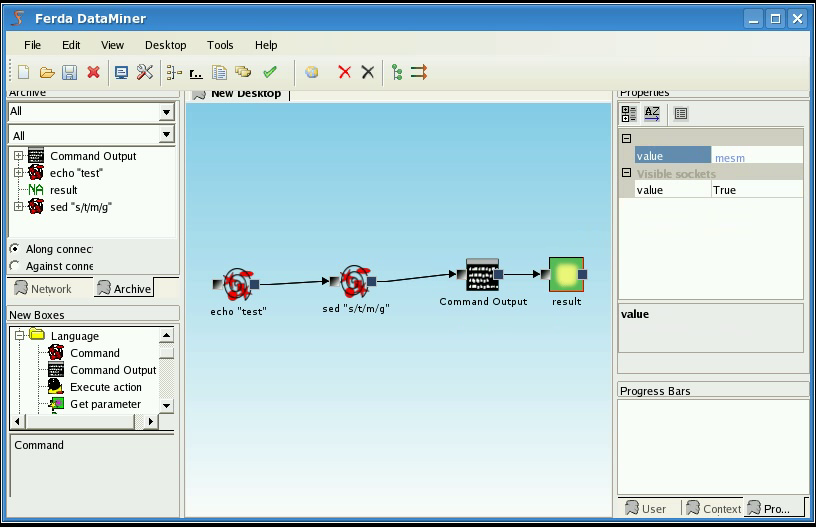
\includegraphics[width=1\textwidth]{command2.png}
	\caption{Command and command output}
	\label{fig:boxCommand}
\end{figure}

\begin{figure}
	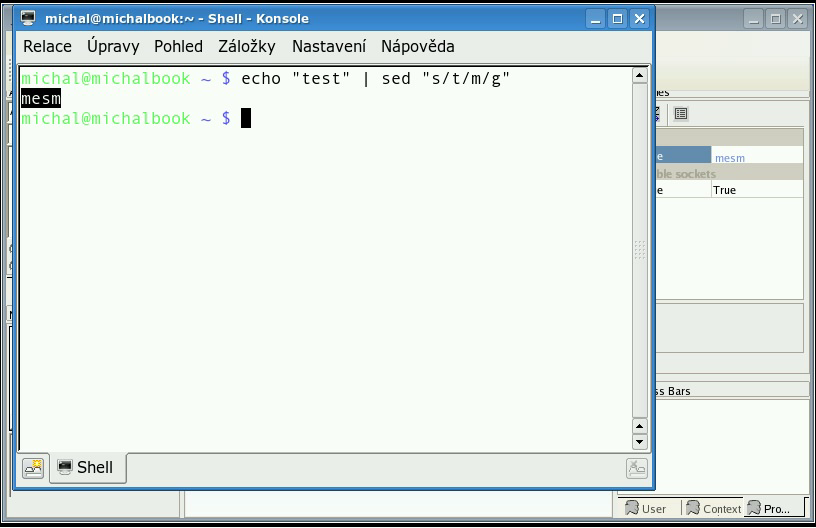
\includegraphics[width=1\textwidth]{command3.png}
	\caption{Konsole version of the previous example}
	\label{fig:CommandKonsole}
\end{figure}

\subsubsection{User-programmable box}
There are two ways how to write a program in the Ferda language. First way is to use only predefined boxes. The second way is to create own boxes and use them in the final program. The first scenario is typical for standard users of the system. The second can be used by advanced programmers. For the latter scenario it is necessary to know the Ferda system in detail.

Let us think about box whose functionality can be programmed in some standard scripting language in the time of running Ferda. Such box can have several properties which specify number of sockets, their names and types of boxes which can be connected to those sockets. The next property should be a string property which specifies the program of the box. For such box we would prefer Python as the programming language, because of its strength and cause Ice has a good support for it.

Such box would add a quicker way how to program a new functionality without having deep knowledge of the Ferda system. 

\section{Advanced tools and topics}

\subsection{Unit tests}
For developers in general it is useful to have some framework for testing of units of their programs. Programmers of the Ferda system would like to be able to make sure quickly that their changes in the system do not affect the programs in the Ferda language or affect them exactly in the way they expect. Programmers in the Ferda language would like to know that their programs works as expected.

Creation of a box called ``UnitTest'' would take profit. The box should have a name and one socket for connecting ``Assert'' boxes. Assert box should be a box which validates some condition and when the condition is not satisfied it should return a message describing the problem. Then there should be a small application which takes a project as parameter and calls all unit tests in the project. Unit tests should call all asserts which are connected to the test. When any of them fails the application should return the message with the name of the unit test and the error message from the failed assert. Even if one unit test failed it should call other tests.

Similar is the NUnit framework for .NET Framework. For reusing tools which execute NUnit tests it would be nice to create a generator of NUnit tests from the Ferda project unit tests. Such generator should create one assembly for one project, but also as many test methods as many unit test boxes there are in the project. There should be one startup method for initializing the Ferda Project Manager and for loading a project. 

\subsection{Distributed computation}
Ferda uses Ice for communication among its parts. Every box module can reside on different computer. Placement of box module is specified before execution of Ferda. It means that during the runtime user is not able to change where which box is running and is not able to create two instances of one box module which would run on two different computers. This means that for example it is not possible to load data from first computer, process them on second and save results on third one. 

However, Ferda could be extended in that point. Ferda uses for finding box modules the IceGrid service. This service supports multiple identical box modules on different computers. The modules manager could load all these box modules and add to every box a virtual property ``placement'' which gives the users the ability to choose placement of instance of the box. If user changed this property, old instance could be removed from connections and destroyed, a new instance with the same parameters would be created and added to the connections. Such process would be transparent from the user's perspective.

If the user opened a project on different computer and the placement property were set to a computer which is not managed by IceGrid of the new computer, Ferda could take as a placement any of the available placements. IceGrid supports several load balancing algorithms which could be also used for setting up the new placement.

\chapter{KDD problems and their solutions}
\label{chap:KDDExamples}
This chapter shows data-mining examples and shows how they can be solved in the Ferda system by functionalities introduced in the previous chapters. It also proposes new functionalities specific for knowledge discovery.

\section{Fourfold task in a recursion}
\subsection{Motivation}
Changes to a setting of a data-mining task are often needed after having the knowledge of found patterns of the task. Subsequent run of that task can result in next changes to that settings. This step is repeated until the analyst is satisfied with the patterns or they give up that setting at all. It is manual and confusing.

It is possible that the analyst has an algorithm how to change a setting after run of a task according to patterns. Such information should be expressible in the Ferda language. If it is done the algorithm can be reused or adjusted to different tasks.

Let us get a fourfold task setting with the founded implication quantifier. Generally, if the threshold of the founded implication is too high, no results are returned by the task. If the threshold of the founded implication is too low many meaningless patterns are returned.

We will present small program in the new language which finds threshold for founded implication so that the count of patterns of a task which use that quantifier is between specified numbers.

\subsection{Implementation}
The solution is based on linear interpolation. The function of a count of patterns on a threshold is non-increasing. If we know two thresholds (the $x_{min}$ and the $x_{max}$) with their count of patterns (the $y_{min}$ and the $y_{max}$) where $y_{max}$ is smaller than what we want and $y_{min}$ is greater than what we want, then we can interpolate this way: 

\begin{math}
x = x_{max} - (y_{max} - y)\frac{x_{max} - x_{min}}{y_{max} - y_{min}}
\end{math}

, where $y$ is the wanted count of patterns. Please see figure~\ref{fig:linearInterpolationPlot}. Such new $x$ is then lesser or equal to $x_{max}$ and greater or equal to $x_{min}$. Such computation would be repeated.

\begin{figure}
	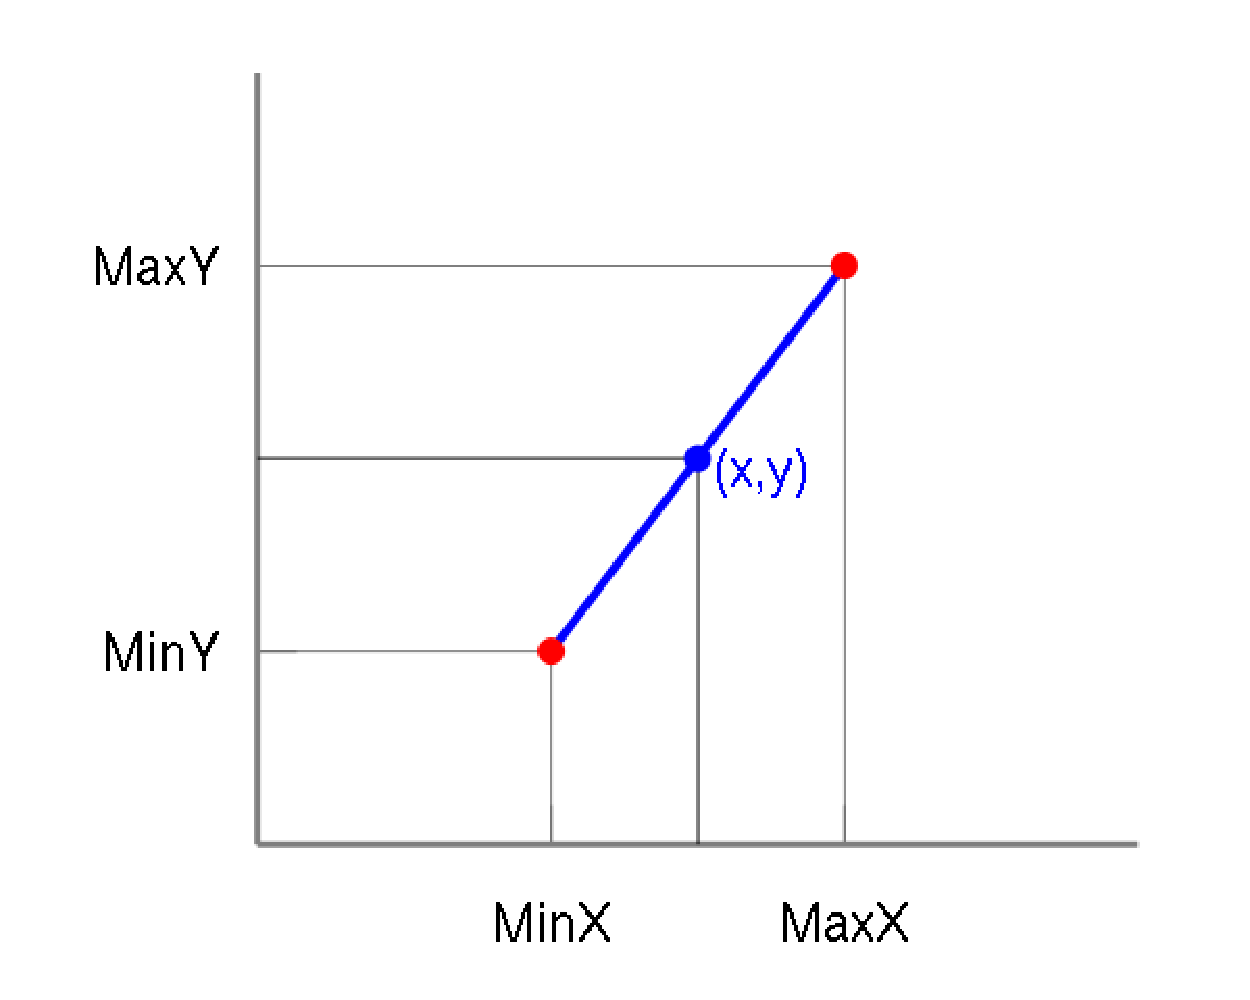
\includegraphics[width=1\textwidth]{linearInterpolationPlot}
	\caption{linear interpolation plot}
	\label{fig:linearInterpolationPlot}
\end{figure}

Because the function of a count of patterns on a threshold is not continuous we can not be sure that such interpolation founds the wanted count of patterns. To overcome this the program searches for a short interval, rather than for one number. In the present example we are showing, $y$ (wanted number of patterns) is set to 5, but it will be satisfied if the count of patterns is between 2 and 10. It is still not enough, but it is simple and it helps. We can count in the program how deep it is in recursion and stop it after several steps if it does not find a sufficient result. But we will not do that for leaving the program as simple as it can be. It is not hard to do that with the new language, you can try it as an exercise. 

The interpolation can be done in Ferda with the new box binary operation. Please see figure~\ref{fig:linearInterpolationBoxes}. Compare it to the equation above.

\begin{figure}
	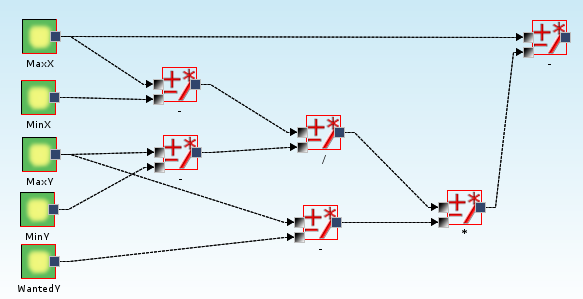
\includegraphics[width=1\textwidth]{linearInterpolation}
	\caption{interpolation as a connection of boxes}
	\label{fig:linearInterpolationBoxes}
\end{figure}

Hence, the program computes repetitively new threshold until it is satisfied. But which numbers should be at the beginning in the $x_{min}$, $x_{max}$, $y_{min}$ and $y_{max}$ variables? Let us make a decision that if a threshold is 1, there are no results. This is true in standard situations. So, we can in the $x_{max}$ put 1 and in the $y_{max}$ put 0. Let us make second decision that if a threshold is 0, the number of results equals to the ``max number of hypotheses'' parameter of the fourfold task. Hence, we can put $x_{min}=0$ and to the $y_{min}$ put the same number as is in the ``max number of hypotheses'' parameter. Such thing can be best done by specifying that count only once in a integer box and connecting them to both ``max number of hypotheses'' socket and the socket of the ``MinY'' box.

At the beginning the threshold will be set to $0.5$. The program will first try to compute the number of patterns for that threshold. If the count is between 2 and 10 the program returns that threshold.   

\begin{figure}
	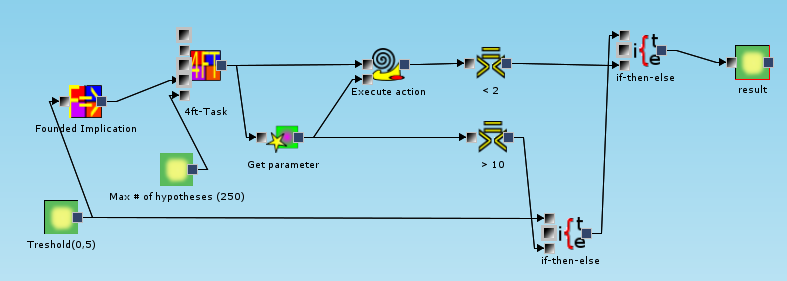
\includegraphics[width=1\textwidth]{exampleMainMiningPart}
	\caption{Basic of the recursive fourfold example}
	\label{fig:basicRecursiveExample}
\end{figure}

Please see figure~\ref{fig:basicRecursiveExample}. The four leftmost boxes specify setting of the fourfold task. The ``Get parameter'' box has set property ``ParameterName'' to ``NumberOfHypotheses''. The ``Execute action'' box has set property ``ActionName'' set to ``Run''. It means that both these boxes return number of hypotheses (patterns) of the setting (they are equal as far as their value is concerned, because ``Get parameter'' box is connected to the ``Function'' socket of the box ``Execute action''). The ``Execute action'' also executes a search for hypotheses in the setting. Without executing the action the count of hypotheses can be invalid. So the action must be at least once executed. Two ``IfThenElse'' boxes with two ``Comparison'' boxes in the figure return the actual threshold if the number of hypotheses is between 2 and 10.

\begin{figure}
	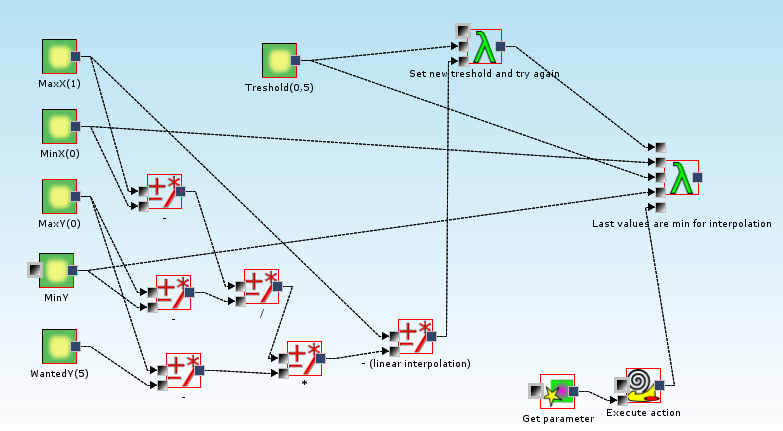
\includegraphics[width=1\textwidth]{exampleMainRecursionPart}
	\caption{Result should be between}
	\label{fig:resultBetween}
\end{figure}

If the number of hypotheses is smaller than 2 or greater than 10 the program will compute by interpolation a new threshold and executes this again. Please see figure~\ref{fig:resultBetween}. This is a part of the program where the count of hypotheses is greater than 10. In the interpolation $x_{min}$ will be set to the last threshold, $y_{min}$ will be set to the last count of hypotheses. Than a new threshold will be computed by the interpolation and the result will be again connected to the ``IfThenElse'' box from the previous figure. You can see the both sub-connections together in figure~\ref{fig:exampleWithoutInterpolationOnMax}.

\begin{figure}
	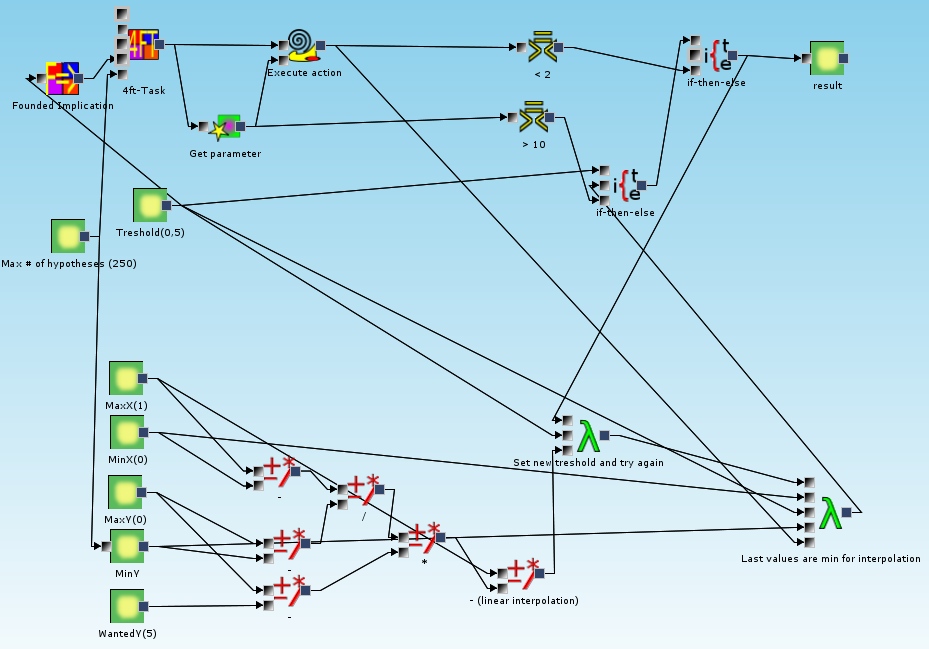
\includegraphics[width=1\textwidth]{exampleWithoutInterpolationOnMax}
	\caption{Example without $NumberOfHypotheses < 2$ part}
	\label{fig:exampleWithoutInterpolationOnMax}
\end{figure}

Whole program without details of fourfold settings can be seen in figure~\ref{fig:exampleResult}. There is also a part of the program for the variant where the count of hypotheses is smaller than 2. You can see that the connection do not look nice. It is because of tangle of lines in the figure. Users can collapse boxes by a packing feature of FrontEnd. They can also use more desktops for organizing the program. A similar program in standard imperative languages would not be easier.

\begin{figure}
	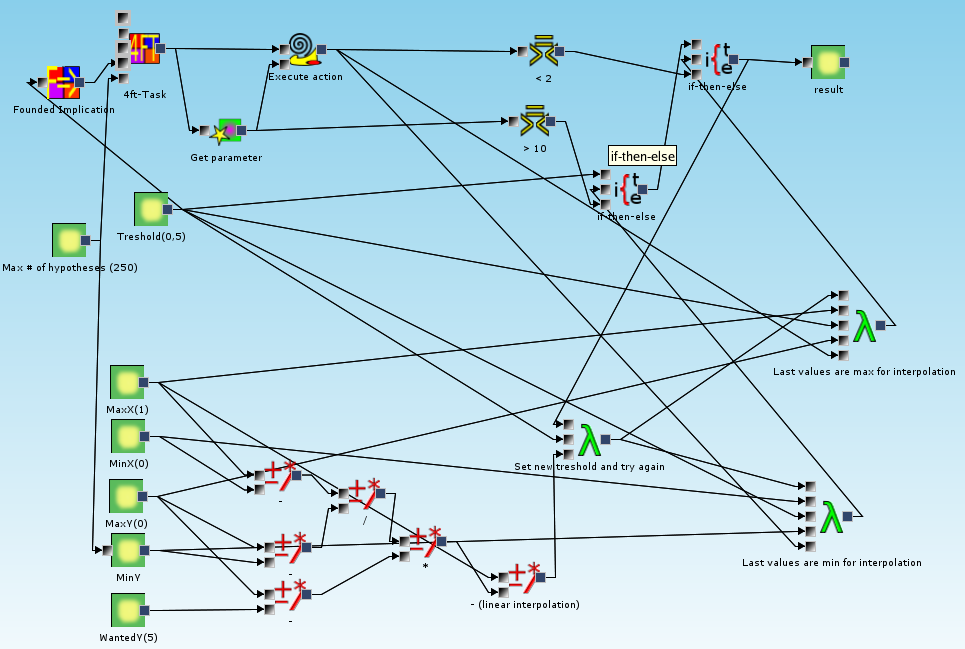
\includegraphics[width=1\textwidth]{exampleResult}
	\caption{Whole example}
	\label{fig:exampleResult}
\end{figure}

!-- TODO predelat obrazky ``Treshold'' na ``Threshold'', a misto ``Execute action'' snad muze byt zapojena do lambd krabicka ``Get parameter'' - tedy dost to zrychli pocitani (mozna je potreba jeste pres double box a je mi divne, ze bych to nezkousel -- mozna v tom je nejaky figl, zkusim) --!

\subsection{How to do it better}
The recursive computation is not needed for this particular task. The BestN algorithm for tasks, which is outlined in \cite{thesisKuchar}, can solve this particular task more efficiently. But a user has to be able to specify what results are the most appropriate. A functional language is a strong tool for such thing. We can see a functional language as a superset of observational calculi, which are described in~\cite{GUHAbook}. If we have only one quantifier, which is fuzzy, it is easy to sort results according to goodness. For example, if we have only founded implication, a formula with higher threshold is better. Founded implication is not fuzzy today, still we can convert it to that easily.

Two or more quantifiers as a setting for a task are more complicated. The today's tasks accept a formula if all its quantifiers are satisfied. Hence the formula can be seen as a conjunction of the same sub-formulas only with a different quantifier. That conjunction is the real quantifier which is used in the GUHA mining. That conjunction should be used as a sorting filter for BestN. Today we have problem that the conjunction used is not a fuzzy conjunction. There is only one or zero. But there are many different fuzzy conjunctions and the user should have the ability to choose the right conjunction. They should be able to writetheir own conjunctions by the programming language.

There can be still more complicated tasks where the recursive solution described here can be useful.

\section{Getting basic information from a table}
Sometimes you get data and know hardly anything about it. In such situations it would be convenient to have a method how to get quickly basic information about it.

A program which creates a basic generic settings from a table without any knowledge about it will be presented in this section. We will focus rather on a way how the user can create such program than on particular quantifiers, tasks and other properties of a setting which it should use.

Let us create a fourfold task setting which has in the antecedent all atom settings created from all columns of the table. Hence, the program should create an attribute for all columns in the table. It should decide on the type of the attribute depending on the data in the column. Similarly, it should create an atom setting from the attribute. All these atom settings should be included in the cedent for the fourfold task.

The program would create a sequence of atom settings for all columns. But first let us describe how we would write a function which returns a sequence of all columns of a table in Ferda. The table box type should have a new read-only property with names of columns. Today such information is returned by a method of a functions interface of the table box. The only way how to get such information from functions is by a custom box. If we had a property with columns names, let us call it ``columns'', the GetParameter box could be used for getting such information as a parameter to a next box. The map box is the box we would used as the next box.

\begin{eqnarray*}
Map(&&What=GetParameter(name="columns", box=Table(\dots)), \\&& Do=Column(name=X, table=Table(\dots)), \\&& Variable=X)
\end{eqnarray*}

This connection returns a sequence of columns. The $X$ can represent for example $String()$ or $Variable()$.

The second task is to create an attribute which depends on values in a column. If the column had more than 20 distinct values the \emph{equifrequency} attribute would be used, otherwise the \emph{each value one category} attribute would be used. Let us call the column in previous connection $C$

\begin{eqnarray*}
C=Column(name=X, table=Table(\dots))
\end{eqnarray*}

Then if we changed in the last connection in the Map box the connection to the ``Do'' socket this way

\begin{eqnarray*}
Do=IfThenElse(&&Comparasion(type="<=", \\&&\qquad value1=GetParameter(name="distinctValues", \\&&\qquad\qquad box=C), \\&&\qquad value2=20),\\&&Atom(EachValueOneAttribute(column=C,\dots)),\\&&Atom(EquifrequencyAttribute(column=C,\dots)))
\end{eqnarray*}

result of such connection would be the wanted sequence of atom settings. Such sequence could be connected to a cedent box, which could be then connected as both the antecedent and the succedent of a fourfold task.

\section{GUHA in Ferda by ``small'' boxes}
In this section the generic GUHA-Method written in the Ferda language is described. It presents only really basic concepts, it provides neither an implementation of the method nor a detailed description.

The principle of GUHA procedures is simple: Let us have set of formulas in an observational calculus~\cite{GUHAbook}. Go trough all these formulas and return those which are valid on a specific data.

If we wanted to create a generic GUHA-Method, the formulas of the observational calculus would be representable in the Ferda language. Because the calculus is similar to functional language the implementation would not be so hard. Predicates, junctors and quantifiers would be separate boxes.

If we had representable formulas of the observational calculus, we would have the possibility to create a set of such formulas. The sequence boxes, which are described in section~\ref{sec:sequences}, would be handy for this task. Specific boxes for generating a sequence of formulas would be also useful.

The next problem is computation which formulas are valid. Because formula is a function, it should be only computing of the function on a specific data. This is simple.

The last problem is how to show the results. A new result browser for generic GUHA-Method would be needed.

Such GUHA-Method would bring big amount of new questions which can be asked against data compared to the actual implementation, but such implementation would be slower. For scientific purposes it can be really useful.

\chapter{Summary}
The thesis has described a new language for data mining. It is a visual functional language. Functions are there called boxes. Basic formalization of the language has been shown in section~\ref{sec:formalisation}. A source code is written as a connection of boxes, source files are project files of the Ferda system. Possible extensions to source files has been described in section~\ref{sec:reusability}. These extensions add better reusability of code. One such extension, which is called ``network archive'', has been implemented as a part of this thesis. The network archive is a new place where users can store connections. It is independent of projects. One network archive can be accessed from more computers. It is a way how to move connections from one project to another. Future possible enhancement to the network archive has been also proposed.

A basic set of boxes has been created as a part of the thesis and other boxes have been proposed. The boxes which has been created include the constant boxes, the BinaryOperation box, the Comparison box, the IfThenElse box, the Lambda box, the GetParameter box, the ExecuteAction box, the Command box and the CommandOutput box. The most complicated box from these is the Lambda box. There has been discussed several problems of the box and their possible solutions. The boxes which have been only proposed include various sequence boxes and the user-programmable box.

Three examples of the usage of the new language for data-mining has been shown. The first example introduces a recursive computation of data mining tasks. An implementation of that example is a part of this thesis. The second example shows how a generic setting which gets basic information about data in any table can be created with the proposed language. The third example presents a more generic implementation of the GUHA principle based on simple boxes.

%\section{Future tasks to do in Ferda}
%popis jednotlivych tasku s narocnosti, uzitkem - bodove ohodnotit

% modules for interacion je treba vylepsit

%\bibliographystyle{abbrv}
%\bibliographystyle{czechiso}

%\bibliographystyle{abbrvnat}

\bibliographystyle{cj}
\bibliography{thesis}

%\begin{thebibliography}{thesisKuchar}
%\bibitem{GMGC} Rauch J., Šimůnek M.: GUHA Method and Granular Computing. In: Hu X., Liu Q., Skowron A., Lin T. Y., Yager R., Zang B. (ed.). Proceedings of IEEE konference Granular Computing 2005. Piscataway: IEEE, 2005, s. 630–635. ISBN 0-7803-9017-2.
%\bibitem{thesisKuchar} Tomáš Kuchař -- jeho diplomová práce
%\bibitem{GUHAbook} GUHA book
%\bibitem{znalosti2006} Kováč M., Kuchař T., Kuzmin A., Ralbovský M.: Ferda, nové vizuální prostředí pro dobývání znalostí. Přijato k prezentaci na konferenci ZNALOSTI 2006, viz http://fim.uhk.cz/znalosti/index.php?p=prispevky
%\bibitem{Ice} Internet Communications Engine documentation
%\bibitem{Wiki} linearni interpolace 
%\bibitem{dalsi} \dots
%\end{thebibliography}
\end{document}
